% PREAMBLE
\documentclass[11pt]{amsart}
\usepackage[T1]{fontenc}
\usepackage{lmodern}
\usepackage{microtype}
\usepackage{amsmath,amssymb}
\usepackage{mathtools}
\usepackage{graphicx}
\usepackage{booktabs}
\usepackage{tikz}
\usepackage[colorlinks=true,linkcolor=blue!45!black,citecolor=blue!45!black,urlcolor=blue!45!black]{hyperref}
\usepackage[capitalize]{cleveref}

\emergencystretch=1.5em

\newtheorem{theorem}{Theorem}[section]
\newtheorem{proposition}[theorem]{Proposition}
\newtheorem{lemma}[theorem]{Lemma}
\newtheorem{corollary}[theorem]{Corollary}
\newtheorem{conjecture}[theorem]{Conjecture}
\theoremstyle{definition}
\newtheorem{definition}[theorem]{Definition}
\newtheorem{fact}[theorem]{Fact}
\theoremstyle{remark}
\newtheorem{remark}[theorem]{Remark}

\title{The Even Half of the Slice Sign Law}
\author{Carlo Mitchener}
\address{MrlyProd, Inc.}
\email{carlo.mitchener@gmail.com}
\date{First published 2026-08-31, revised 2026-09-02}

% PAPER
\begin{document}

\begin{abstract}
Slice a sponge along its longest diagonal, count the cells the cut meets, and watch how fast that count grows as the sponge is refined; the growth rate lands just above or just below the value a generic slice would give, and which side it lands on is decided by nothing but whether the dimension is even or odd. That is the sign law. Its odd half was proved in a companion paper. This paper proves the even half at the two smallest odd bases: on the middle-digit design in base $3$ and in base $5$, the Perron root $\rho_D$ of the carry matrix satisfies $\rho_D < f_D/q$ for every even $D \ge 2$, where $f_D$ is the fill of the digit polynomial, so the diagonal slice exponent sits strictly below the generic value in every even dimension. Both proofs run on one machine: an exact Fourier form of the Collatz--Wielandt test vector, an exact telescoping in which the leading fill-powers cancel identically, and a frequency-separation estimate. The two bases differ only in how deep the certificate must go. Base $5$ needs depth $\Theta(\log D)$; base $3$ needs depth $\Theta(D^2)$, and the quadratic transient is identified: its length is $\tfrac14 (\log R)\, D^2 + O(D)$ with $R = \prod_{i \ge 2} \cos(\pi/3^i)/\cos(2\pi/3^i)$ and $\tfrac14\log R = 0.0568486146\ldots$, the crossing of the half-point frequency. A one-line lemma explains why base $3$ alone is hard: it is the unique odd base at which the design's digit-generating polynomial has the same modulus at $-1$ as at $1$. Exact integer certificates settle bases $7$, $9$ and $11$ on stated finite ranges with depth at most two and no transient at all. The second half of the paper turns to what the sign law still lacks -- strictness at odd $D \equiv 1 \pmod 3$ -- and reduces it to a $2$-adic bound whose first layer is a proved tent law built from the Jacobsthal numbers.
\end{abstract}

\begin{center}

\includegraphics[width=0.36\textwidth]{figures/avatar.png}
\end{center}
\maketitle

% INTRODUCTION

\section{Introduction}
\label{sec:intro}

Take a cube, cut it into $27$ equal subcubes, and throw away the seven that touch the middle of a face or the middle of the cube. Twenty survive. Repeat inside each survivor forever and you get the Menger sponge. Now cut the sponge with the plane through its centre perpendicular to a main diagonal, and count how many little cubes the plane meets at each stage of the construction. That count is a sequence of integers, and this paper is about how fast it grows.

The same question makes sense in every dimension, and in every odd base. Fix an odd base $q$ and let $m = (q-1)/2$ be its middle digit. In the $D$-dimensional base-$q$ grid, keep a cell exactly when at most one of its $D$ digits equals $m$. At $q = 3$ and $D = 3$ this is the Menger sponge; at general $D$ it is the $D$-dimensional analogue. Cut along the main diagonal, count the cells the cut meets at level $L$, and call that count $b_D(L)$. It grows geometrically, and the growth rate is the Perron root $\rho_D$ of a finite integer matrix, the \emph{carry matrix}, which we build in \cref{sec:defs}.

There is an obvious guess for $\rho_D$. The whole solid at level $L$ has $f_D^{\,L}$ cells, where $f_D$ is the number of admissible digit vectors in one step. A hyperplane is a codimension-one slice, so a generic slice should meet about $f_D^{\,L}/q^L$ of them, and the guess is $\rho_D = f_D/q$. The guess is never right. The truth is a law:

\begin{center}
\emph{$\rho_D > f_D/q$ at odd $D$, and $\rho_D < f_D/q$ at even $D$.}
\end{center}

The diagonal slice is not generic in any dimension, and the side it misses on is decided by the parity of $D$ alone. We call this the \emph{sign law}. The odd half of it -- $\rho_D > f_D/3$ for every odd $D$, strictly whenever $D \not\equiv 1 \pmod 3$ -- was proved in the companion paper \cite{slice-order}, where it falls out of a single pointwise inequality: at odd $D$ the design symbol is raised to an even power, so a certain trigonometric sum is nonnegative term by term and the census can only run ahead of $(f_D/q)^L$.

At even $D$ that argument inverts and dies. The symbol acquires an odd power, the trigonometric sum changes sign, and no pointwise estimate survives; \cref{sec:certs} records the precise obstruction. This paper proves the even half anyway, at the two smallest odd bases.

\begin{figure}[ht]
\centering
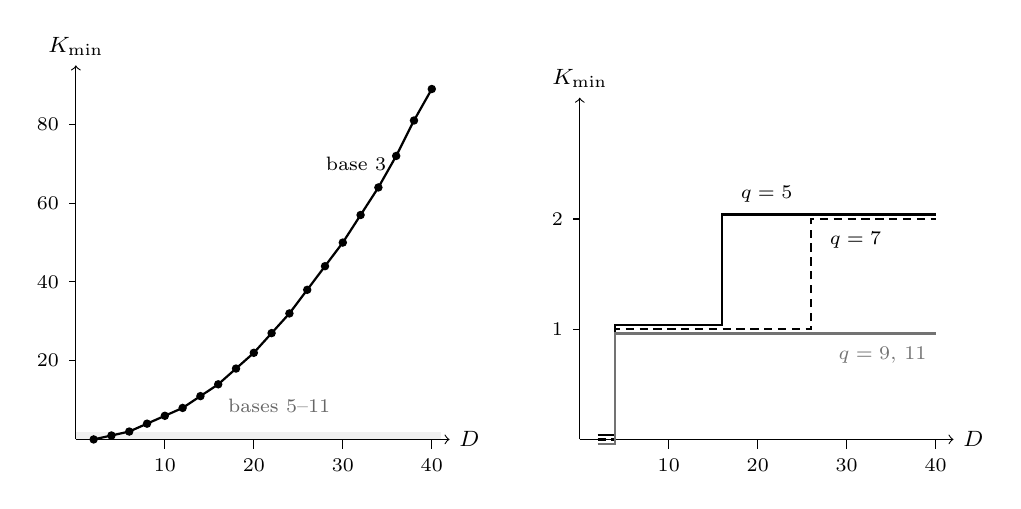
\begin{tikzpicture}
\begin{scope}[x=0.113cm, y=0.05cm]
  \fill[black!6] (0,0) rectangle (41,2);
  \draw[->] (0,0) -- (42,0) node[right, font=\footnotesize] {$D$};
  \draw[->] (0,0) -- (0,95) node[above, font=\footnotesize] {$K_{\min}$};
  \foreach \x in {10,20,30,40} \draw (\x,0) -- (\x,-2.5) node[below, font=\scriptsize] {$\x$};
  \foreach \y in {20,40,60,80} \draw (0,\y) -- (-0.8,\y) node[left, font=\scriptsize] {$\y$};
  \draw[thick] plot[mark=*, mark size=1.1pt] coordinates {(2,0) (4,1) (6,2) (8,4) (10,6) (12,8) (14,11) (16,14) (18,18) (20,22) (22,27) (24,32) (26,38) (28,44) (30,50) (32,57) (34,64) (36,72) (38,81) (40,89)};
  \node[font=\scriptsize, anchor=west] at (27,70) {base $3$};
  \node[font=\scriptsize, anchor=west, black!60] at (16,8.5) {bases $5$--$11$};
\end{scope}
\begin{scope}[shift={(6.4cm,0cm)}, x=0.113cm, y=1.4cm]
  \draw[->] (0,0) -- (42,0) node[right, font=\footnotesize] {$D$};
  \draw[->] (0,0) -- (0,3.1) node[above, font=\footnotesize] {$K_{\min}$};
  \foreach \x in {10,20,30,40} \draw (\x,0) -- (\x,-0.09) node[below, font=\scriptsize] {$\x$};
  \foreach \y in {1,2} \draw (0,\y) -- (-0.8,\y) node[left, font=\scriptsize] {$\y$};
  \draw[thick] plot[const plot] coordinates {(2,0.04) (4,1.04) (16,2.04) (40,2.04)};
  \draw[thick, densely dashed] plot[const plot] coordinates {(2,0) (4,1) (26,2) (40,2)};
  \draw[thick, black!55] plot[const plot] coordinates {(2,-0.04) (4,0.96) (40,0.96)};
  \node[font=\scriptsize, anchor=south west] at (17,2.06) {$q=5$};
  \node[font=\scriptsize, anchor=north west] at (27,1.97) {$q=7$};
  \node[font=\scriptsize, anchor=north west, black!55] at (28,0.93) {$q=9,\,11$};
\end{scope}
\end{tikzpicture}
\caption{Certificate depth $K_{\min}$ against even dimension $D$, at bases $3$, $5$, $7$, $9$ and $11$, every value an exact integer computation. The depth is how many steps of the carry matrix a proof of $\rho_D < f_D/q$ needs before the inequality becomes visible. Left: base $3$ pays a quadratic transient, with $K_{\min}$ growing like $D^2$; the pale strip is $K \le 2$, where every other base lives. Right: that strip magnified - the staircases of bases $5$, $7$, $9$ and $11$ never exceed depth $2$ on the ranges computed here, stepping later as the base grows; the steps of bases $9$ and $11$ to depth $2$ sit at $D = 42$ and $D = 60$, just beyond the plotted range. \Cref{sec:base3} identifies the base-$3$ constant exactly and \cref{lem:unique} says why base $3$ is alone.}
\label{fig:depth}
\end{figure}

\medskip
\noindent\textbf{The results.} \Cref{thm:base5}: on the base-$5$ middle-digit design, $\rho_D < f_D/5$ for \emph{every} even $D \ge 2$. \Cref{thm:base3}: on the base-$3$ middle-digit design, $\rho_D < f_D/3$ for \emph{every} even $D \ge 2$. The odd half at base $3$ is \cite{slice-order}; \cref{prop:oddhalf} below records the same argument base-free, which supplies the odd half at base $5$ as well. So the sign law now holds in sign at every dimension at base $3$ and at base $5$, with only one gap left anywhere: strictness in the exceptional odd residue classes.

\medskip
\noindent\textbf{How.} Both theorems run on one machine, and it is a small one. A Collatz--Wielandt test vector $\beta_K$, obtained by pushing the all-ones vector $K$ steps through the transposed carry matrix, certifies $\rho_D < f_D/q$ the moment $q\beta_{K+1} < f_D \beta_K$ holds componentwise. That is a finite, exact, integer test, and it gives strictness for free -- no determinant lemma, no exceptional class. The work is showing that some $K$ always exists, and \cref{fig:depth} is the shape of that work. In an exact Fourier form $\beta_K$ becomes a sum over frequencies $n$ modulo $q^{K}$, the leading fill-powers cancel identically, and the certificate reduces to positivity of a single explicit trigonometric sum $\Sigma_K$ on a window of carries. At base $5$ one frequency dominates all others by a uniform factor $0.768$ per unit of $D$, and depth $K(D) = \Theta(\log D)$ closes everything. At base $3$ a second frequency -- the one riding the fixed point $\pi$ of angle tripling -- fights the first at comparable strength, wins for a while, and only loses at depth $\Theta(D^2)$. That fight is the transient, and \cref{thm:transient} pins its length to within one odd step of a closed form.

\medskip
\noindent\textbf{The second theme.} Proving $\rho_D \ne f_D/q$ on the odd side, in the residue classes where the easy rational-root argument is silent, turns out to be a $2$-adic question about $\det M_{\mathrm{even}}$, and the answer has a shape nobody expected: the mod-$2$ nullity of the even core is a tent function built out of the Jacobsthal numbers $J(k) = (2^k - (-1)^k)/3$ \cite{oeisA001045}. The second half of the paper proves that tent law, computes the next Smith layer, and states the remaining bound as \cref{b:con:V}, the valuation gap. The algebra underneath the layers is a syzygy module of three polynomials, which puts it squarely in classical territory -- $\mu$-bases and the degree identity \cite{csc98,dohm}, the predictable-degree property \cite{forney}, Toeplitz kernel structure \cite{heinig}, polynomial-matrix normal forms \cite{dopico,lindy} -- and the second half is careful to say which parts are borrowed and which are not.

\medskip
\noindent\textbf{What is not new.} Carry chains for adding $D$ numbers in base $q$ are classical, and their transition matrix is Holte's amazing matrix \cite{holte}, whose eigenvalues are $1, q^{-1}, \dots, q^{-(D-1)}$ and whose eigenvectors are known in closed form. Collatz--Wielandt is a textbook criterion. The $D = 3$ base-$3$ diagonal slice count of the companion paper matches OEIS \href{https://oeis.org/A299916}{A299916} \cite{oeisA299916} up to an index shift, the Menger reading there being a user comment on the entry. What is new is the even half of the sign law itself, at both bases, uniformly in $D$; the exact Fourier form of the certificate vector and its telescoping; the frequency-separation bound; the identification of the base-$3$ transient constant $\tfrac14\log R$; and \cref{lem:unique}, the one-line reason base $3$ is the only difficult base.

% DEFINITIONS

\section{The design, the census, and the carry machine}
\label{sec:defs}

Throughout, $q \ge 3$ is an odd integer, $m = (q-1)/2$ is its middle digit, and $D \ge 2$ is the dimension. All three are fixed unless a statement says otherwise.

\begin{definition}[the design]
\label{def:design}
A digit vector $(d_1,\dots,d_D) \in \{0,\dots,q-1\}^D$ is \emph{admissible} when at most one $d_i$ equals $m$. The level-$L$ solid is the set of cells of the $q^L$-refined $D$-dimensional grid all of whose $L$ digit vectors are admissible. At $q = 3$, $D = 3$ this is the Menger sponge; at $q = 3$ and general $D$ it is the $D$-dimensional Menger analogue.
\end{definition}

\begin{definition}[digit polynomial and fill]
\label{def:poly}
Let $A_q(t) = \sum_{d \ne m} t^d$ and
\[
  P_D(t) = A_q(t)^{D-1}\bigl(A_q(t) + D\,t^m\bigr),
\]
so that $P_D[s]$ is the number of admissible digit vectors of coordinate sum $s$. The \emph{fill} is $f_D = P_D(1) = (q-1)^{D-1}(q-1+D)$, the number of admissible digit vectors. At $q = 3$ the polynomial factors as
\[
  P_D(t) = (1+t^2)^{D-1}\bigl(1 + Dt + t^2\bigr), \qquad f_D = 2^{D-1}(D+2).
\]
\end{definition}

The factorisation is a two-line count: either no coordinate takes the middle digit, or exactly one of $D$ does.

\begin{fact}
\label{fact:poly}
$P_D$ agrees with brute-force enumeration of all $q^D$ digit tuples, and the base-$3$ factorisation of \cref{def:poly} holds, for bases $3$ and $5$ and every $2 \le D \le 8$. Verified by \texttt{check\_polynomials} in \texttt{scripts/verify.py}.
\end{fact}

\begin{lemma}[palindromy and positivity]
\label{lem:palin}
$\deg P_D = D(q-1) = 2Dm$ and $P_D[Dm + x] = P_D[Dm - x]$ for every $x$; moreover $P_D[s] > 0$ for every $0 \le s \le D(q-1)$.
\end{lemma}

\begin{proof}
The digit set $\{0,\dots,q-1\}$ is symmetric about $m$, and so is $\{0,\dots,q-1\}\setminus\{m\}$, so $A_q[d] = A_q[q-1-d]$, i.e. $t^{q-1}A_q(1/t) = A_q(t)$. Since $q-1-m = m$ we also have $t^{q-1}\bigl(A_q(1/t) + D t^{-m}\bigr) = A_q(t) + D t^m$. Multiplying the $D-1$ copies of the first relation by the one copy of the second gives $t^{D(q-1)}P_D(1/t) = P_D(t)$, which is the stated palindromy about $Dm$. For positivity, the second factor has every coefficient on $\{0,\dots,q-1\}$ at least $1$, and the support of $A_q^{D-1}$ contains $\{0, q-1, 2(q-1),\dots,(D-1)(q-1)\}$ because $q \ge 3$ puts both $0$ and $q-1$ in the support of $A_q$. Given $s$, set $j = \min\bigl(\lfloor s/(q-1)\rfloor, D-1\bigr)$; then $0 \le s - j(q-1) \le q-1$ and $P_D[s] \ge A_q^{D-1}[j(q-1)] \cdot (A_q + Dt^m)[s-j(q-1)] > 0$.
\end{proof}

\begin{definition}[census]
\label{def:census}
The level-$L$ census $b_D(L)$ counts the admissible level-$L$ cells whose coordinate sum is congruent to the \emph{palindromic centre} $Dm(1 + q + \dots + q^{L-1}) = D(q^L-1)/2$ modulo $q^L$. This is the central diagonal hyperplane together with its $q^L$-translates; $b_D(0) = 1$.
\end{definition}

\begin{definition}[carry automaton and carry matrix]
\label{def:carry}
Read digits least significant first. A level-$L$ history of digit-vector sums $(s_0,\dots,s_{L-1})$ meets the census condition exactly when the carries $c_0 = 0$, $c_{j+1} = (c_j + Dm - s_j)/q$ are all integers. Accordingly set
\[
  M = M^{(D)}, \qquad M[c',c] = P_D[\,c + Dm - q c'\,],
\]
with \emph{row index the new carry and column index the old carry}, acting on column vectors by $u_{L+1} = M u_L$, $u_0 = e_0$. Then $u_L(c)$ counts the level-$L$ histories with terminal carry $c$, and $b_D(L) = \mathbf{1}^{\top} M^L e_0$. Orientation is load-bearing: every statement below about ``sums of $M$'' means \emph{column} sums in this orientation.
\end{definition}

\begin{lemma}[carry window and forward closure]
\label{lem:window}
Every carry reachable from $0$ satisfies $\lvert c \rvert \le \lfloor (D-1)/2 \rfloor$, and the state set $S = \{c : \lvert c\rvert \le \lfloor (D-1)/2\rfloor\}$ is forward closed: $M[c',c] \ne 0$ with $c \in S$ forces $c' \in S$. We write $M$ for the restriction to $S$; the even core defined below has size $n = \lceil D/2 \rceil$ at both parities, and $n$ always means that size.
\end{lemma}

\begin{proof}
$M[c',c] \ne 0$ requires $0 \le c + Dm - qc' \le D(q-1) = 2Dm$, i.e. $(c-Dm)/q \le c' \le (c+Dm)/q$. For $\lvert c \rvert \le \lfloor (D-1)/2\rfloor$ this gives $\lvert c' \rvert \le \lfloor (D-1)/2 \rfloor$, since $\bigl(\tfrac{D-1}{2} + Dm\bigr)/q = \tfrac{D}{2} - \tfrac{1}{2q} < \tfrac{D}{2}$, and the only integers of modulus $< D/2$ are those of modulus $\le \lfloor (D-1)/2 \rfloor$. The reachability statement is the same computation started at $c_0 = 0$.
\end{proof}

\begin{lemma}[reflection and the even core]
\label{lem:core}
$M[-c',-c] = M[c',c]$, so the carry reflection $R: c \mapsto -c$ commutes with $M$. The orbit of $u_0 = e_0$ lies in the $+1$ eigenspace of $R$, of dimension $\lceil D/2 \rceil$; the restriction of $M$ to that eigenspace is the \emph{even core} $M_{\mathrm{even}}$, an $n \times n$ integer matrix with $n = \lceil D/2 \rceil$. The characteristic polynomial factors as $\chi_M = \chi_{M_{\mathrm{even}}}\chi_{M_{\mathrm{odd}}}$.
\end{lemma}

\begin{proof}
$M[-c',-c] = P_D[-c + Dm + qc'] = P_D[Dm - (c - qc')] = P_D[Dm + (c-qc')] = M[c',c]$ by \cref{lem:palin}. Since $R$ commutes with $M$ and $Re_0 = e_0$, every $u_L$ is reflection-even. Splitting $\mathbb{R}^S$ into the $\pm 1$ eigenspaces of $R$ is an $M$-invariant decomposition, which is the factorisation of $\chi_M$.
\end{proof}

\begin{fact}
\label{fact:fold}
$\det M = \det M_{\mathrm{even}} \cdot \det M_{\mathrm{odd}}$ exactly, at bases $3$ and $5$ and every $D \le 25$. Verified by \texttt{check\_fold} in \texttt{scripts/verify.py}.
\end{fact}

\begin{proposition}[the core is primitive]
\label{prop:core}
$M$ restricted to $S$ is irreducible and aperiodic; its Perron root is $\rho_D = \rho(M_{\mathrm{even}})$, and $\rho(M_{\mathrm{odd}}) < \rho_D$.
\end{proposition}

\begin{proof}
Aperiodicity is immediate: $M[0,c] = P_D[c + Dm] > 0$ for every $c \in S$ by \cref{lem:palin}, since $0 < c + Dm < 2Dm$; in particular $M[0,0] > 0$ is a self-loop at the state $0$, which every state reaches in one step. Irreducibility takes one line at every odd $q$: for $0 \le c \le \lfloor(D-1)/2\rfloor - 1$ one has $Dm - (q-1)c \ge \tfrac32(q-1) \ge q$, so $0 \le c + Dm - q(c+1) \le 2Dm$ and $M[c+1,c] > 0$ by \cref{lem:palin} -- the carry climbs from $0$ one step at a time to the window edge, the negative states follow by the reflection symmetry of \cref{lem:core}, and every state returns to $0$ in one step. With the self-loop, $M$ on $S$ is primitive. For the spectral statement, $M$ has a nonnegative Perron eigenvector $v$; its even part $(v + Rv)/2$ is nonnegative and nonzero, hence an eigenvector of $M_{\mathrm{even}}$ at $\rho(M)$, so $\rho(M_{\mathrm{even}}) = \rho(M) =: \rho_D$; and by primitivity every other eigenvalue of $M$ has modulus strictly below $\rho_D$, so $\rho(M_{\mathrm{odd}}) < \rho_D$.
\end{proof}

We use \cref{prop:core} only where a growth rate has to be read off the census, namely \cref{thm:reduction}(iii) and \cref{prop:oddhalf}. The certificate theorems of \cref{sec:certs}, and therefore \cref{thm:base5} and \cref{thm:base3}, need none of it.

\begin{definition}[symbol and circle form]
\label{def:symbol}
Let $g_q(\psi) = 2\sum_{j=1}^{m}\cos(j\psi) = \dfrac{\sin(q\psi/2)}{\sin(\psi/2)} - 1$, the Dirichlet kernel with the middle digit removed, and $\Phi_D(\psi) = g_q(\psi)^{D-1}\bigl(D + g_q(\psi)\bigr)$. Both are real and even. Then $A_q(e^{i\psi}) = e^{im\psi}g_q(\psi)$ and $P_D(e^{i\psi}) = e^{imD\psi}\Phi_D(\psi)$. At $q = 3$, $g_3(\psi) = 2\cos\psi$.
\end{definition}

\begin{lemma}[the root of unity, and where parity lives]
\label{lem:rootunity}
$g_q(2\pi t/q) = -1$ for every $t \not\equiv 0 \pmod q$, hence $\Phi_D(2\pi t/q) = (-1)^{D-1}(D-1)$.
\end{lemma}

\begin{proof}
$\sum_{d=0}^{q-1}z^d = 0$ for any $z^q = 1$ with $z \ne 1$; by \cref{def:symbol} that sum is $z^m(1 + g_q)$ and $z^m \ne 0$, so $g_q = -1$. Then $\Phi_D = (-1)^{D-1}(D-1)$.
\end{proof}

This single value is the whole parity mechanism. It is the design symbol evaluated at a nontrivial $q$-th root of unity, and it carries the factor $(-1)^{D-1}$ that flips the sign law.

\begin{proposition}[what the sign law says]
\label{prop:mass}
Let $w > 0$ be the right Perron vector of $M$ on $S$, normalised to $\sum_c w_c = 1$, and let $p_D = \sum_{q \mid c} w_c$ be its mass on carries divisible by $q$. Then
\[
  q\,\rho_D = f_D + (-1)^{D-1}(D-1)\bigl(q\,p_D - 1\bigr),
\]
which at $q = 3$ reads $3\rho_D = f_D + (-1)^{D-1}(D-1)(3p_D-1)$. Consequently the sign law at every dimension and both parities at once is equivalent to the single parity-free inequality $p_D > 1/q$.
\end{proposition}

\begin{proof}
The column sum of $M$ at $c$ is $\sum_{s \equiv c + Dm \ (q)} P_D[s]$. Root-of-unity filtering with $\omega = e^{2\pi i/q}$ turns this into $q^{-1}\sum_{t}\omega^{-t(c+Dm)}P_D(\omega^t)$; by \cref{def:symbol} and \cref{lem:rootunity} the $t = 0$ term is $f_D$ and every other term is $(-1)^{D-1}(D-1)\omega^{tmD}$, so all phases collapse to $\omega^{-tc}$ and
\[
  \sum_{c'}M[c',c] = \tfrac{1}{q}\Bigl(f_D + (-1)^{D-1}(D-1)\bigl(q\,\mathbf{1}[q\mid c] - 1\bigr)\Bigr).
\]
Contract against $w$, using $\rho_D = \mathbf 1^{\top}Mw$ and $\mathbf 1^{\top}w = 1$. The sign statement follows because $(-1)^{D-1}(D-1) > 0$ at odd $D$ and $< 0$ at even $D$, and the factor $q p_D - 1$ never changes sign with $D$.
\end{proof}

\begin{remark}[what Holte's matrix does and does not give]
\label{rem:holte}
Add $D$ base-$q$ numbers digit by digit with independent uniform digits and the carries form a Markov chain whose transition matrix is Holte's ``amazing matrix'' \cite{holte}: spectrum exactly $1, q^{-1}, \dots, q^{-(D-1)}$, stationary vector the Eulerian numbers, eigenvectors known in closed form as Foulkes characters and Eulerian idempotents \cite{df09,df12}. Our matrix departs from that frame in two independent ways, and both matter. First, the design of \cref{def:design} restricts digit vectors \emph{jointly across coordinates} -- at most one coordinate may carry the middle digit -- so $P_D$ is not a product of $D$ one-coordinate factors; the published generalisations of the carries process vary the digit set, to shifted consecutive sets and negative bases \cite{ns14} and to balanced digits \cite{df14}, but all keep the summands' digits independent, and all keep the $q^{-j}$ spectrum. Second, the outgoing digit is \emph{pinned} rather than summed over, because the census of \cref{def:census} fixes a hyperplane: the entry of $M$ is a single coefficient of $P_D$ where Holte's is a sum of $q$ consecutive coefficients, so $M$ is not stochastic, and its column sums are the root-of-unity filter computed in \cref{prop:mass}. Undo both departures and one recovers $q^D$ times Holte's matrix exactly, on his recurrent states and in his indexing, once orientation is fixed: his row index is the incoming carry, so his $P(i,j)$ corresponds to our column-incoming $M[j,i]$. His chain also lives on $0, \dots, D-1$ where ours uses the centred window of \cref{lem:window}: the difference is his transient top state plus our reflection fold, not a different automaton. Keep the two departures and the classical spectrum is destroyed outright -- already at $q = 3$, $D = 3$ the even core is $\bigl(\begin{smallmatrix}6&6\\1&3\end{smallmatrix}\bigr)$ with the irrational Perron root $(9+\sqrt{33})/2$, which no rescaling of an integer spectrum can produce. That is why the questions of this paper are open rather than quotable. We are not aware of any treatment in the carries literature of jointly restricted digits, nor of any arithmetic study -- reduction mod $p$, Smith normal form, $p$-adic elementary divisors, rank or nullity -- of a carry matrix of any kind; the second half of this paper is such a study.
\end{remark}

% CERTIFICATES

\section{The reduction and the two certificate machines}
\label{sec:certs}

This section is short and entirely proved. It reduces the sign law to a statement about one integer sequence, and then gives two finite tests, either of which settles a single dimension outright.

Write $\hat u_L(\psi) = \sum_c u_L(c)e^{ic\psi}$, let $m_0(L) = \sum_{c \equiv 0 \ (q)}u_L(c)$, and set
\[
  V(L) = q\,m_0(L) - b_D(L), \qquad W_k = q^{k-1}\bigl(q\,b_D(k) - f_D\,b_D(k-1)\bigr).
\]

\begin{theorem}[the reduction chain]
\label{thm:reduction}
Let $q \ge 3$ be odd and $D \ge 2$. Then:
\begin{enumerate}
\item[(i)] \emph{(transfer recursion, exact phase cancellation)} for every $L \ge 0$ and every real $\psi$,
\[
  \hat u_{L+1}(\psi) = \frac1q\sum_{r=0}^{q-1}\Phi_D(y_r)\,\hat u_L(y_r), \qquad y_r = \frac{\psi + 2\pi r}{q};
\]
\item[(ii)] \emph{(step identity)} for every $k \ge 1$, $\;W_k = (-1)^{D-1}(D-1)\,q^{k-1}\,V(k-1)$; in particular at even $D$, $\;q\,b_D(L+1) - f_D\,b_D(L) = -(D-1)V(L)$;
\item[(iii)] \emph{(eventual contraction)} if $D$ is even and $V(L) \ge 0$ for every $L \ge L_0$, then $\rho_D \le f_D/q$.
\end{enumerate}
\end{theorem}

\begin{proof}
(i) By \cref{def:carry}, $\hat u_{L+1}(\psi) = \sum_{c'}e^{ic'\psi}\sum_c P_D[c + Dm - qc']\,u_L(c)$. Insert the indicator $[q \mid N] = q^{-1}\sum_{r<q}e^{2\pi i rN/q}$ with $N = c + Dm - s$, then reindex the inner sum by $s$, so that $c' = N/q$ and $c'\psi + 2\pi rN/q = Ny_r$. The two exponentials merge and
\[
  \hat u_{L+1}(\psi) = \frac1q\sum_{r<q}\hat u_L(y_r)\cdot e^{iDm\,y_r}P_D(e^{-iy_r}).
\]
By \cref{def:symbol} with $\psi \mapsto -y_r$ and evenness of $\Phi_D$, $P_D(e^{-iy_r}) = e^{-imDy_r}\Phi_D(y_r)$, so $e^{iDm y_r}P_D(e^{-iy_r}) = \Phi_D(y_r)$ and every phase is gone.

The cancellation deserves a sentence in words. The symbol carries the phase $e^{imD\psi}$ because $P_D$ is palindromic about $Dm$ (\cref{lem:palin}); the carry rule carries the offset $+Dm$ at every level because the census target of \cref{def:census} \emph{is} the palindromic centre. These are the same $Dm$, and they cancel identically -- not asymptotically, not up to a unimodular constant. Move the census target off centre and the recursion still closes, but no longer on real even data.

(ii) Put $\psi = 0$ in (i), so $y_r = 2\pi r/q$ and $b_D(L+1) = \hat u_{L+1}(0)$. The $r = 0$ term is $q^{-1}f_D\,b_D(L)$. For $r \ne 0$, \cref{lem:rootunity} makes $\Phi_D(2\pi r/q) = (-1)^{D-1}(D-1)$, a constant, and
\[
  \sum_{r \ne 0}\hat u_L(2\pi r/q) = \sum_c u_L(c)\bigl(q\,\mathbf 1[q \mid c] - 1\bigr) = q\,m_0(L) - b_D(L) = V(L).
\]
Hence $q\,b_D(L+1) - f_D\,b_D(L) = (-1)^{D-1}(D-1)V(L)$; multiply by $q^{k-1}$ at $L = k-1$.

(iii) By (ii) at even $D$, $V(L) \ge 0$ gives $b_D(L+1) \le (f_D/q)\,b_D(L)$ for every $L \ge L_0$, so $b_D(L) \le C\,(f_D/q)^L$ with $C = b_D(L_0)(q/f_D)^{L_0}$. By \cref{prop:core} the core is primitive, so $b_D(L)^{1/L} = \bigl(\mathbf 1^{\top}M^Le_0\bigr)^{1/L} \to \rho_D$, and therefore $\rho_D \le f_D/q$.
\end{proof}

\begin{fact}
\label{fact:reduction}
The step identity of \cref{thm:reduction}(ii) holds in exact integer arithmetic at bases $3$, $5$ and $7$, for every $D \le 12$ and every $k \le 6$. Verified by \texttt{check\_reduction} in \texttt{scripts/verify.py}.
\end{fact}

\begin{remark}[why even $D$ is genuinely harder]
\label{rem:obstruction}
At odd $D$ the exponent $D-1$ is even, so $\Phi_D \ge 0$ pointwise and every $W_k \ge 0$ term by term; that is the whole odd-half proof of \cite{slice-order}. At even $D$ the sign of $\Phi_D$ follows the sign of $g_q$, and the needed inequality is false pointwise: already at $q = 3$ and $k = 2$, the quantity $W_2/\bigl((-1)^{D-1}(D-1)\bigr)$ is negative for every even $D \ge 6$, because the term at angle $8\pi/9$ outweighs the two positive ones. No pointwise-positivity certificate and no magnitude-only certificate can work at even $D$. What follows is built to survive that.
\end{remark}

The odd half is the other side of that same remark, and \cref{thm:reduction} states it base-free. We record it because \cref{b:sec:strict} needs the odd half at base $5$ and \cite{slice-order} proves it only at base $3$. The argument is that paper's and is not new here.

\begin{proposition}[the odd half, non-strict, at any odd base]
\label{prop:oddhalf}
Let $q \ge 3$ be odd and let $D \ge 3$ be odd with $D + g_q(\psi) > 0$ for every real $\psi$. Then $\rho_D \ge f_D/q$. The hypothesis holds for every odd $D \ge q$, since $g_q(\psi) = 2\sum_{j \le m}\cos(j\psi) \ge -2m = -(q-1)$; at $q = 3$ it holds for every odd $D \ge 3$, since $g_3 \ge -2$; and at $q = 5$ it holds for every odd $D \ge 3$, since $g_5(\psi) = 4\cos^2\psi + 2\cos\psi - 2 \ge -9/4$, the minimum at $\cos\psi = -1/4$.
\end{proposition}

\begin{proof}
At odd $D$ the exponent $D-1$ is even, so $g_q^{D-1} \ge 0$ and $\Phi_D = g_q^{D-1}(D + g_q) \ge 0$ pointwise. Now $\hat u_0 \equiv 1 \ge 0$, and \cref{thm:reduction}(i) writes $\hat u_{L+1}(\psi)$ as a nonnegative combination of values of $\hat u_L$, so $\hat u_L \ge 0$ on all of $\mathbb R$ for every $L$ by induction. In particular $V(L) = \sum_{r \ne 0}\hat u_L(2\pi r/q) \ge 0$, computed in the proof of \cref{thm:reduction}(ii). That same identity at odd $D$ reads $q\,b_D(L+1) - f_D\,b_D(L) = (D-1)V(L) \ge 0$, so $b_D(L) \ge (f_D/q)^L$ for every $L$, and $b_D(L)^{1/L} \to \rho_D$ by \cref{prop:core}.
\end{proof}

\begin{theorem}[the row certificate]
\label{thm:row}
Fix $D$ and let $v_c = q\,\mathbf 1[q \mid c] - 1$, so that $V(L) = v^{\top}u_L$. Suppose there is an integer $t \ge 1$ with
\[
  \bigl(v^{\top}M^{t}\bigr)_j \ge 0 \ \text{ for every } j \in S, \qquad\text{and}\qquad V(L) \ge 0 \ \text{ for } L = 0,\dots,t-1.
\]
Then $V(L) \ge 0$ for every $L \ge 0$; hence, at even $D$, $\rho_D \le f_D/q$ by \cref{thm:reduction}(iii).
\end{theorem}

\begin{proof}
Three lines. For $L \ge t$, $V(L) = v^{\top}M^{t}u_{L-t} = \sum_j\bigl(v^{\top}M^t\bigr)_j\,u_{L-t}(j)$. The vector $u_{L-t}$ is entrywise nonnegative because $u_0 = e_0 \ge 0$ and $M \ge 0$. Both factors are nonnegative, so the sum is. For $L < t$ the hypothesis is the prefix check.
\end{proof}

The row certificate is cheap -- one matrix power and one sign scan -- but it proves only $\rho_D \le f_D/q$, and turning $\le$ into $<$ then costs a determinant argument with an exceptional residue class. The second machine avoids that entirely.

\begin{theorem}[the column certificate, Collatz--Wielandt]
\label{thm:column}
Let $\beta_K = (M^{\top})^K\mathbf 1$, that is $\beta_K(c) = \sum_{c'}(M^K)[c',c]$, the number of level-$K$ histories \emph{started} at carry $c$, with $\beta_0 = \mathbf 1$. Then $\beta_K > 0$ on $S$ for every $K \ge 0$, and if for some $K \ge 0$
\[
  q\,\beta_{K+1}(c) < f_D\,\beta_K(c) \qquad\text{for every } c \in S,
\]
then $\rho_D < f_D/q$, strictly.
\end{theorem}

\begin{proof}
Positivity: every carry in $S$ has at least one admissible successor in $S$ by \cref{lem:window} and \cref{lem:palin}, so the column sums of $M^K$ are positive. For the criterion, recall the strict Collatz--Wielandt bound: if $B \ge 0$ and $x > 0$ satisfy $Bx < \theta x$ componentwise, then with $\theta' = \max_i (Bx)_i/x_i < \theta$ one gets $B^kx \le \theta'^kx$, so every entry of $B^k$ is at most $\theta'^k(\max x)/(\min x)$ and $\rho(B) \le \theta' < \theta$. Apply it with $B = M^{\top}$, $x = \beta_K$, $\theta = f_D/q$, noting $M^{\top}\beta_K = \beta_{K+1}$. Finally $\rho(M^{\top}) = \rho(M) = \rho_D$.
\end{proof}

Two features of \cref{thm:column} matter for everything that follows. It gives \emph{strict} inequality with no determinant lemma and no exceptional class, and it does not care where the test vector came from: any positive integer vector passing the componentwise test is a proof. The whole of \cref{sec:base5} and \cref{sec:base3} is the construction of a $K$ at which $\beta_K$ passes.

\begin{remark}[the depth is not free]
\label{rem:depthzero}
$K = 0$ never works for $D > 1$: the test reads $f_D + (-1)^{D-1}(D-1)\bigl(1 - q\,\mathbf 1[q\mid c]\bigr) < f_D$, which at even $D$ fails at every $c$ with $q \nmid c$. That one line is the entire difficulty of the even case: the all-ones vector is off by exactly the $(D-1)$ of \cref{lem:rootunity}, and the certificate must smooth it away.
\end{remark}

% BASE FIVE

\section{Base 5: the even half entire}
\label{sec:base5}

\begin{theorem}[the even half at base $5$]
\label{thm:base5}
On the base-$5$ middle-digit design ($q = 5$, $m = 2$), $\rho_D < f_D/5$ for every even $D \ge 2$, where $f_D = 4^{D-1}(D+4)$. Equivalently, the diagonal slice exponent lies strictly below the generic value $\log_5 f_D - 1$ in every even dimension.
\end{theorem}

The proof occupies the rest of this section. Standing notation: $D$ is even, $S = \{\lvert c\rvert \le (D-2)/2\}$, and $\beta_K$ is as in \cref{thm:column}, extended to all $c \in \mathbb{Z}$ by the same formula. The extension is harmless: $S$ is forward closed by \cref{lem:window}, so the restricted and unrestricted towers agree on $S$.

\begin{proposition}[Fourier form]
\label{prop:fourier5}
For every $K \ge 0$, $\beta_K$ is $5^K$-periodic and
\[
  \beta_K(c) = 5^{-K}\sum_{n \bmod 5^K} F_K(n)\,e^{2\pi i nc/5^K}, \qquad F_K(n) = \prod_{i=1}^{K}\Phi_D\bigl(2\pi n/5^i\bigr).
\]
\end{proposition}

\begin{proof}
Induction on $K$; $K = 0$ is $\beta_0 = \mathbf 1$. Assume the formula at $K$. Then $\beta_{K+1}(c) = \sum_{c'}M[c',c]\beta_K(c')$; insert the indicator $[5 \mid N] = \tfrac15\sum_{r<5}e^{2\pi irN/5}$ with $N = c + 2D - s$ \emph{before} substituting the inductive hypothesis, and write $\theta = 2\pi(n + r5^K)/5^{K+1}$. The two exponentials merge, and the inner sum over $s$ is $e^{i(c+2D)\theta}P_D(e^{-i\theta}) = e^{ic\theta}\Phi_D(\theta)$ by \cref{def:symbol} with $mD = 2D$ -- the same identical cancellation as in \cref{thm:reduction}(i), now iterated. As $(n,r)$ runs over $\mathbb{Z}/5^K \times \mathbb{Z}/5$, $N' = n + r5^K$ runs over $\mathbb{Z}/5^{K+1}$ exactly once, and $\Phi_D(2\pi N'/5^i) = \Phi_D(2\pi n/5^i)$ for $i \le K$ since the arguments differ by a multiple of $2\pi$. Hence $F_K(n)\Phi_D(\theta) = F_{K+1}(N')$.
\end{proof}

\begin{proposition}[exact telescoping]
\label{prop:tele5}
For even $D$ and every $K \ge 0$,
\[
  f_D\,\beta_K(c) - 5\,\beta_{K+1}(c) = 5^{-K}(D-1)\,\Sigma_K(c),
\]
where, with $T_K(n) = \prod_{i=2}^{K+1}\Phi_D(2\pi n/5^i)$,
\[
  \Sigma_K(c) = \sum_{\substack{n \bmod 5^{K+1} \\ 5 \nmid n}} T_K(n)\,e^{2\pi inc/5^{K+1}} = 2\!\!\sum_{\substack{1 \le n < 5^{K+1}/2 \\ 5 \nmid n}}\!\! T_K(n)\cos\!\bigl(2\pi nc/5^{K+1}\bigr),
\]
real and $5^{K+1}$-periodic in $c$. Consequently the depth-$K$ hypothesis of \cref{thm:column} is \emph{equivalent} to
\[
  (C_K): \qquad \Sigma_K(c) > 0 \quad\text{for every } \lvert c\rvert \le (D-2)/2.
\]
\end{proposition}

\begin{proof}
Split the sum of \cref{prop:fourier5} at level $K+1$ by divisibility. For $5 \mid n$, writing $n = 5n'$, one has $F_{K+1}(5n') = \Phi_D(2\pi n')F_K(n') = f_D\,F_K(n')$ and $e(5n'c/5^{K+1}) = e(n'c/5^K)$, so that block of $\beta_{K+1}$ is \emph{exactly} $(f_D/5)\beta_K$. This is an identity, not an estimate: it is the entire leading-order cancellation. For $5 \nmid n$, \cref{lem:rootunity} gives $\Phi_D(2\pi n/5) = -(D-1)$ at even $D$, so $F_{K+1}(n) = -(D-1)T_K(n)$; two minus signs give the stated sign. Reality is evenness of $\Phi_D$, and the paired form comes from $n \leftrightarrow 5^{K+1}-n$. The equivalence is immediate since $5^{-K} > 0$ and $D - 1 > 0$.
\end{proof}

The frequency $n = \pm 1$ leads, and the next lemma says by how much, uniformly in $K$. Write $\hat g_i = g_5(2\pi/5^i)$, $Q_K(n) = \prod_{i=2}^{K+1}\lvert g_5(2\pi n/5^i)\rvert$, so $\lvert T_K(n)\rvert = Q_K(n)^{D-1}\prod_i\lvert D + g_i\rvert$, and note $T_K(1) > 0$ because every angle $2\pi/5^i$ with $i \ge 2$ lies in $(0,\pi/2)$.

\begin{lemma}[frequency separation]
\label{lem:sep5}
For every $K \ge 1$ and every $n \bmod 5^{K+1}$ with $5 \nmid n$ and $n \not\equiv \pm 1$,
\[
  Q_K(n)/Q_K(1) \;\le\; r := 0.768 .
\]
\end{lemma}

\begin{proof}
Let $j = \min\{i \ge 2 : n \not\equiv \pm 1 \bmod 5^i\}$, finite by hypothesis. For $i < j$ we have $n \equiv \varepsilon \bmod 5^i$ with a single sign $\varepsilon$ -- consistent because $5^{i-1} > 2$ forces the signs at consecutive levels to agree -- so $2\pi n/5^i \equiv \pm 2\pi/5^i \pmod{2\pi}$ and $\lvert g_5(2\pi n/5^i)\rvert = \hat g_i$ \emph{exactly}: those factors contribute $1$. For $i > j$ use $\lvert g_5 \rvert \le 4$, so their total contribution is at most $C_j = \prod_{i>j}4/\hat g_i$, which converges: $g_5(x) \ge 4 - 5x^2$ gives $4/\hat g_i \le \bigl(1 - a\,25^{-i}\bigr)^{-1}$ with $a = \tfrac54(2\pi)^2$, and $\prod_{i>j}(1-x_i)^{-1} \le \bigl(1 - \sum x_i\bigr)^{-1}$. In certified interval arithmetic $C_2 \le 1.0033008$ and $C_3 \le 1.0001317$. Three branches remain, indexed by $j$.
\begin{itemize}
\item $j = 2$: enumerating the eighteen residues $n \bmod 25$ with $5 \nmid n$, $n \not\equiv \pm1$, gives $\lvert g_5(2\pi n/25)\rvert \le 2.8242670$, attained at $n = \pm 2$, against $\hat g_2 \ge 3.6897796$. The ratio is $\le 0.7654303$, and times $C_2$ at most $0.7679580$.
\item $j \ge 3$: here $n \equiv \varepsilon \bmod 5^{j-1}$ and $n \not\equiv \varepsilon \bmod 5^j$, so $n \equiv \varepsilon + t\,5^{j-1} \bmod 5^j$ with $t \in \{1,2,3,4\}$, i.e. $2\pi n/5^j = 2\pi t/5 \pm 2\pi/5^j$: the distance to the nearest $2\pi t/5$ is exactly one grid unit, never more. Since $g_5(2\pi t/5) = -1$ by \cref{lem:rootunity} and $\lvert g_5'\rvert \le 6$, we get $\lvert g_5(2\pi n/5^j)\rvert \le 1 + 12\pi/5^j$, which against $\hat g_j \ge 4 - 5(2\pi/5^j)^2$ and times $C_j$ is at most $0.3264722$ at $j = 3$ and at most $0.2651481$ for $j \ge 4$.
\end{itemize}
The maximum of the three branches is $0.7679580 < 0.768$.
\end{proof}

Every numerical constant in that proof, and in \cref{prop:crit5,lem:exit3,lem:subtree3,lem:cross3} and the proofs of \cref{thm:base5,thm:base3} below, is a rigorous rational-interval evaluation with outward rounding on every operation, re-certified by \texttt{scripts/certify.py}; \cref{sec:repro} names the block that carries each one. Nothing in this paper rests on a floating-point evaluation.

The bound is uniform in $K$ and within $1.3\%$ of the truth: the exact maxima are $0.75818$ at $K = 2$, $0.75789$ at $K = 3$ and $0.75788$ at $K = 4$, all attained at $n \equiv \pm 2$.

\begin{proposition}[the criterion]
\label{prop:crit5}
Let $D \ge 6$ be even, $K \ge 1$, and $\kappa(D,K) = \dfrac{D+4}{D+\hat g_2}\Bigl(\dfrac{D+4}{D+\hat g_3}\Bigr)^{K-1}$. If
\[
  \bigl(2\cdot 5^K - 1\bigr)\,r^{D-1}\,\kappa(D,K) \;<\; \cos\!\Bigl(\frac{\pi(D-2)}{5^{K+1}}\Bigr) \qquad\text{and}\qquad 5^{K+1} \ge 4(D-2),
\]
then $(C_K)$ holds, hence $\rho_D < f_D/5$.
\end{proposition}

\begin{proof}
The window condition $5^{K+1} \ge 4(D-2)$ and $\lvert c \rvert \le (D-2)/2$ give $\lvert 2\pi c/5^{K+1}\rvert \le \pi(D-2)/5^{K+1} \le \pi/4$, so the $n = \pm1$ term of $\Sigma_K(c)$ is at least $2T_K(1)\cos\bigl(\pi(D-2)/5^{K+1}\bigr) > 0$. Counting the remaining frequencies: there are $(5^{K+1}-1)/2$ integers in $[1, 5^{K+1}/2)$, of which $(5^{K+1}-5)/10$ are multiples of $5$, leaving $2\cdot 5^K$, and excluding $n=1$ leaves $2\cdot 5^K - 1$. For each, $\lvert T_K(n)\rvert/T_K(1) = \bigl(Q_K(n)/Q_K(1)\bigr)^{D-1}\prod_{i=2}^{K+1}\lvert D + g_i\rvert/(D+\hat g_i)$. In that second product the factors with $i < j$ are exactly $1$, because the $g$-values themselves agree there and not merely their moduli; the remaining at most $K$ factors are each $\le (D+4)/(D+\hat g_i) \le (D+4)/(D+\hat g_3)$ for $i \ge 3$, and the largest admissible shape is the $j = 2$ one, which is $\kappa(D,K)$. We need $D + g_i \ge D - 4 > 0$, hence $D \ge 6$. Combine with \cref{lem:sep5} and the triangle inequality.
\end{proof}

\begin{proof}[Proof of \cref{thm:base5}]
Take $K(D) = \min\{K \ge 1 : 5^{K+1} \ge 4(D-2)\}$, and split.

\emph{Even $18 \le D \le 32$.} Here $K(D) = 2$ and the criterion of \cref{prop:crit5} is checked directly with certified interval constants: the left-hand sides are $0.5594$, $0.3296$, $0.1942$, $0.1144$, $0.0674$, $0.0398$, $0.0234$, $0.0138$ against right-hand sides $0.9202$, $0.8994$, $0.8763$, $0.8510$, $0.8235$, $0.7940$, $0.7624$, $0.7290$. Eight inequalities, all strict.

\emph{Even $D \ge 34$.} First, $4(D-2) \ge 128 > 25 = 5^2$, so $K(D) \ge 2$ and $K(D) - 1 \ge 1$ is admissible; minimality then gives $5^{K} < 4(D-2)$, whence $2\cdot 5^K - 1 < 8(D-2) < 8D$ and $K < \log_5(4D)$. The window condition gives right-hand side $\ge \cos(\pi/4)$. By $1 + x \le e^x$,
\[
  \kappa(D,K) \le B(D) := \Bigl(1 + \tfrac{4-\hat g_2}{D + \hat g_2}\Bigr)\exp\Bigl(\tfrac{(4-\hat g_3)(\log_5(4D)-1)}{D+\hat g_3}\Bigr),
\]
and $B$ is decreasing on $D \ge 34$: the first factor visibly is, and the derivative of $(\log_5(4D)-1)/(D+\hat g_3)$ has the sign of $(D+\hat g_3)/(D\ln 5) - (\log_5(4D)-1)$, whose first term decreases to $1/\ln 5$ while the second increases, and which is at most $0.6943 - 2.0524 < 0$ at $D = 34$. With $B(34) \le 1.0089188$ it suffices that $h(D) = D\,r^{D-1} < \cos(\pi/4)/(8B(34))$, and $\cos(\pi/4)/(8B(34)) \ge 0.0876069$; and $h$ decreases for $D > 1/\lvert\ln r\rvert = 3.7884$ with $h(34) \le 0.0056028$.

\emph{Even $D \le 16$.} Exact integer Collatz--Wielandt certificates: $K = 0$ at $D = 2$, $K = 1$ at $D = 4,6,8,10,12,14$, and $K = 2$ at $D = 16$. Each is the componentwise integer inequality of \cref{thm:column} at the stated depth, with no floating point anywhere.

The case split is real, not decorative: at $D = 16$, $K = 2$ the analytic criterion gives $0.9499$ against $0.9387$ and genuinely fails, so $D = 18$ is exactly where it first bites. In all three cases \cref{thm:column} gives $\rho_D < f_D/5$.
\end{proof}

\begin{fact}
\label{fact:cert5}
The exact integer certificate of \cref{thm:column} passes at base $5$ for every even $D \le 40$, at the depths listed above. Verified by \texttt{check\_even\_certificates} in \texttt{scripts/verify.py}, which asserts the full depth staircase ($K = 0$ at $D = 2$, $K = 1$ at $4 \le D \le 14$, $K = 2$ at $16 \le D \le 40$) and additionally the depths at $D = 64, 66, 314, 316$. Beyond the bundled range the same certificate was run at sampled even $D = 62, 70, 80, 100, 120, 158, 200$.
\end{fact}

Depth cannot be held fixed. Since $\beta_K$ has Fourier support in $5^{-K}\mathbb Z$, the dominant term makes $\Sigma_K(c) \sim 2T_K(1)\cos\bigl(2\pi c/5^{K+1}\bigr)$, so a depth-$K$ certificate sees only the carries inside the first quarter-period, and it fails once $(D-2)/2$ reaches $c_0(K) = \lceil 5^{K+1}/4\rceil$.

\begin{proposition}[every fixed depth dies]
\label{prop:death5}
For each fixed $K \ge 1$, $(C_K)$ fails at $c = c_0(K)$ for all sufficiently large even $D$. Hence depth $K$ certifies only finitely many dimensions and the growth $K(D) = \Theta(\log D)$ of \cref{thm:base5} is necessary, not an artefact of the proof.
\end{proposition}

\begin{proof}
By \cref{lem:sep5} the runner-up frequency satisfies $Q_K(n)/Q_K(1) \le r$, so the $n = \pm1$ term beats the sum of all others by a factor $r^{-(D-1)}/(2\cdot 5^K)$ times a factor bounded uniformly in $D$ (namely $\kappa(D,K) \le \kappa(6,K)$ for fixed $K$). That factor exceeds $1/\lvert\cos(2\pi c_0/5^{K+1})\rvert$ for all large $D$, and $\cos(2\pi c_0(K)/5^{K+1}) < 0$ because $5^{K+1}/4$ is never an integer.
\end{proof}

\begin{fact}[the exact deaths]
\label{fact:death5}
At base $5$, depth $K = 1$ passes at every even $4 \le D \le 14$ and fails first at $D = 16$, at $c = \pm 7$; depth $K = 2$ passes through $D = 64$ and fails first at $D = 66$, at $c = \pm 32$; depth $K = 3$ passes at $D = 314$ and fails first at $D = 316$, at $c = \pm 157$ and nowhere else, while depth $4$ passes there. All three death dimensions are pinned by \texttt{check\_even\_certificates} in \texttt{scripts/verify.py} through the asserted depth staircase at $D = 14, 16, 64, 66, 314, 316$; the identities of the first failing carries, $\pm c_0(K)$, are research-side exact computations over the full window $\lvert c\rvert \le (D-2)/2$. Each first-failure dimension is $2c_0(K)+2$ on the nose.
\end{fact}

The three tags here must be kept apart. \Cref{prop:death5} is \emph{proved} for sufficiently large $D$ at each depth. The exact death law $D = 2\lceil 5^{K+1}/4\rceil + 2$ is \emph{verified} at $K = 1, 2, 3$, as \cref{fact:death5} states. That the same formula gives the exact death at every $K \ge 4$ is a \emph{conjecture}; \cref{sec:bases} shows it is already only asymptotically right at base $7$.

% BASE THREE

\section{Base 3: the even half entire}
\label{sec:base3}

\begin{theorem}[the even half at base $3$]
\label{thm:base3}
On the base-$3$ middle-digit design ($q = 3$, $m = 1$), $\rho_D < f_D/3$ for every even $D \ge 2$, where $f_D = 2^{D-1}(D+2)$. Equivalently, the diagonal slice exponent lies strictly below $\log_3 f_D - 1$ in every even dimension.
\end{theorem}

Here $g_3(\psi) = 2\cos\psi$ and $\Phi_D(\psi) = (2\cos\psi)^{D-1}(D + 2\cos\psi)$. \Cref{prop:fourier5} and \cref{prop:tele5} hold verbatim with $5$ replaced by $3$ and $2D$ by $D$: the carry offset $Dm = D$ and the symbol phase $e^{iD\psi}$ cancel identically as before, and
\[
  f_D\,\beta_K(c) - 3\,\beta_{K+1}(c) = 3^{-K}(D-1)\,\Sigma_K(c),
\]
\[
  \Sigma_K(c) = 2\!\!\sum_{\substack{1 \le n < 3^{K+1}/2\\ 3\nmid n}}\!\! T_K(n)\cos\!\bigl(2\pi nc/3^{K+1}\bigr),
\]
with $T_K(n) = \prod_{i=2}^{K+1}\Phi_D(2\pi n/3^i)$, so that the depth-$K$ certificate is again equivalent to $(C_K)$: $\Sigma_K(c) > 0$ on $\lvert c \rvert \le (D-2)/2$. A useful anchor: $\beta_K(0) = b_D(K)$ exactly, so $\Sigma_K(0) = 3^K V(K)$ and the certificate at $c = 0$ reads the census transient directly.

Everything that differs from base $5$ is in the spectrum. Fix a level $i \ge 2$ and write $N = 3^i$. For an admissible residue $k$ (that is $3 \nmid k$) put $a = \min(k, N-k)$, the grid distance to $0$, and $b = \lvert 2k - N\rvert/2$, the grid distance to the half-point; then $\lvert g_3(2\pi k/N)\rvert = 2\cos\bigl(2\pi\min(a,b)/N\bigr)$.

\begin{lemma}[four nested tracks]
\label{lem:tracks3}
(i) The minima are $a = 1$, at $k = \pm 1$, and $b = 1/2$, at $k = h^{\pm} = (N \mp 1)/2$; these four residues are distinct for $i \ge 2$, and every other admissible $k$ has $a \ge 2$ and $b \ge 5/2$, hence $\lvert g_3\rvert \le 2\cos(4\pi/N)$. (ii) Reducing modulo $3^{i-1}$ sends each of $1, N-1, h^{+}, h^{-}$ at level $i$ to the corresponding residue at level $i-1$; consequently a frequency on a track at level $i$ is on the same track at every level $2 \le i' \le i$, and a frequency that leaves a track never returns to any track. (iii) On a $0$-track, $\lvert g_3\rvert = \hat g_i = 2\cos(2\pi/3^i)$ with amplitude $D + \hat g_i$; on a $\pi$-track, $\lvert g_3 \rvert = \tilde g_i = 2\cos(\pi/3^i)$, with $g_3 < 0$ and amplitude $D - \tilde g_i$.
\end{lemma}

\begin{proof}
(i) $a$ ranges over positive integers prime to $3$, so its next value after $1$ is $2$; $2b = \lvert 2k - N\rvert$ is odd because $N$ is odd, and prime to $3$ because $3 \nmid k$, so its next value after $1$ is $5$. Distinctness holds once $N \ge 9$. The off-track bound is $2\cos$ of an angular distance at least $2\pi\cdot 2/N$. (ii) $h^{+}(i) - h^{+}(i-1) = (3^i - 3^{i-1})/2 = 3^{i-1}$, so $h^{+}(i)\equiv h^{+}(i-1)$, and likewise $h^{-}(i) = h^{+}(i)+1 \equiv h^{-}(i-1)$, $1 \equiv 1$, $3^i - 1 \equiv 3^{i-1}-1$. Downward induction gives the first claim, and the never-return statement is its contrapositive. (iii) Direct evaluation; $g_3 < 0$ on the $\pi$ side because the angle is within $\pi/2$ of $\pi$.
\end{proof}

Because tracks are nested, every non-leading frequency has a well-defined \emph{exit level}: the first level at which it leaves the track it was on. This partitions the spectrum into an exit at each level from a $0$-track, an exit at each level from a $\pi$-track, and the two residues $n \equiv 2, 7 \pmod 9$ that were never on a track above level $1$.

\begin{lemma}[the half-point pair]
\label{lem:half3}
Let $n_h = (3^{K+1}-1)/2$. Then $T_K(n_h) = (-1)^K\prod_{i=2}^{K+1}\tilde g_i^{\,D-1}(D - \tilde g_i)$ and $T_K(1) = \prod_{i=2}^{K+1}\hat g_i^{\,D-1}(D + \hat g_i) > 0$, and for integer $c$, $\cos\bigl(2\pi n_h c/3^{K+1}\bigr) = (-1)^c\cos\bigl(\pi c/3^{K+1}\bigr)$. The leader ratio is
\[
  r(D,K) = \frac{\lvert T_K(n_h)\rvert}{T_K(1)} = \prod_{i=2}^{K+1}\Bigl(\frac{\cos(\pi/3^i)}{\cos(2\pi/3^i)}\Bigr)^{D-1}\frac{D - \tilde g_i}{D + \hat g_i}.
\]
\end{lemma}

\begin{proof}
Direct evaluation on the four track residues of \cref{lem:tracks3}(iii); the sign is one negative $g_3$ per level raised to the odd power $D-1$, so $(-1)^{(D-1)K} = (-1)^K$ at even $D$.
\end{proof}

This is the whole difference between the bases. The half-point pair rides the fixed point $\pi$ of angle tripling, and per level it \emph{beats} the dominant frequency in magnitude, by $\cos(\pi/3^i)/\cos(2\pi/3^i) > 1$; it pays for the advantage only in amplitude, by roughly $(D-2)/(D+2)$ per level. Set
\[
  R = \prod_{i \ge 2}\frac{\cos(\pi/3^i)}{\cos(2\pi/3^i)} = 1.2553249438\ldots
\]
so the total magnitude advantage is $R^{D-1}$ and the total amplitude cost is about $\bigl((D-2)/(D+2)\bigr)^{K}$. Its sign alternates with $K$, so it drags $\Sigma_K(0)$ negative at odd $K$ while it leads. That is the transient.

\begin{lemma}[crossing estimates]
\label{lem:cross3}
Write $\ell_i = \log\bigl(\cos(\pi/3^i)/\cos(2\pi/3^i)\bigr) > 0$, $A = \log\bigl((D+2)/(D-2)\bigr)$, and $s_D = \sum_{i\ge2}\bigl[\log\tfrac{D-\tilde g_i}{D-2} - \log\tfrac{D+\hat g_i}{D+2}\bigr]$, all summands positive and both series geometrically convergent. Then exactly
\[
  \log r(D,K) = (D-1)\bigl[\log R - \mathrm{LT}(K)\bigr] - KA + s_D - \mathrm{ST}(D,K),
\]
with positive tails $\mathrm{LT}(K) < 1.9\cdot 9^{-K}$ and $\mathrm{ST}(D,K) < 7\cdot 9^{-K}/(D-2)$. Setting
\[
  K^{*}(D) = \frac{(D-1)\log R + s_D}{\log\bigl((D+2)/(D-2)\bigr)},
\]
one has $r(D,K) < 1$ for $K > K^{*}(D)$, and $K \ge K^{*}(D)+1$ forces $r(D,K) \le (D-2)/(D+2)$.
\end{lemma}

\begin{proof}
Take the logarithm of the finite product in \cref{lem:half3} and add and subtract the full series; the tails are positive, so dropping them raises the bound, which is the safe direction for the last claim. The tail enclosures are $\log\cos$ expansions, certified in interval arithmetic.
\end{proof}

Every frequency that is not one of the four leaders is exponentially small in $D$, uniformly. Two bounds do that work: an exit cost paid at the level where a frequency leaves its track, and a subtree bound for everything it can do afterwards.

\begin{lemma}[exit costs]
\label{lem:exit3}
Measure each per-level weight against the dominant factor at that level. (i) A frequency exiting a $0$-track at level $j \ge 3$ has weight at most $\bigl(u_o(j)/\hat g_j\bigr)^{D-1}$ with $u_o(j) = 2\cos(\pi/3 - 2\pi/3^j)$, and $u_o(j)/\hat g_j$ is maximal at $j = 3$, where it is at most $0.7052518$, decreasing to $1/2$. (ii) A frequency exiting a $\pi$-track at level $j \ge 3$ has weight at most $\bigl(u_h(j)/\hat g_j\bigr)^{D-1}$ with $u_h(j) = 2\cos(\pi/3 - \pi/3^j)$, maximal at $j = 3$ where it is at most $0.6137010$. (iii) The two residues $n \equiv 2, 7 \pmod 9$ have weight at most $0.2266816^{\,D-1}$. Combining a $\pi$-track prefix with its exit, and writing $P_Q(j) = \prod_{i=2}^{j}\cos(\pi/3^i)/\cos(2\pi/3^i) \le R$, the entry weight of a $\pi$-track exit at level $j$ is at most $0.7528157^{\,D-1}$, the maximum being attained at $j = 3$; the three branch constants are $0.7528157$ at $j = 3$, $0.66966$ at $j = 4$ and $0.6419$ for $j \ge 5$.
\end{lemma}

\begin{proof}
From the $+1$ track at level $j-1$ the non-staying digits give residues $1 + d\,3^{j-1}$, $d \in \{1,2\}$, at angles $2\pi d/3 + 2\pi/3^j$; from the $-1$ track they give the conjugate pair at angles $2\pi d'/3 - 2\pi/3^j$. Since $\lvert 2\cos\rvert$ at $2\pi/3 \pm u$ equals $2\cos(\pi/3 \mp u)$, the larger branch is $2\cos(\pi/3 - 2\pi/3^j) = u_o(j)$, and the amplitude is at most $D + u_o(j) < D + \hat g_j$. As $j$ grows $u_o(j)$ decreases to $1$ while $\hat g_j$ increases to $2$, so the ratio decreases and $j = 3$ is the maximum; the value there is a certified interval evaluation. Case (ii) is identical with $h^{+}$ in place of $+1$, offsets $\pi/3^j$ in place of $2\pi/3^j$, and exit angles $\pi/3 - \pi/3^j$, $5\pi/3 - \pi/3^j$. Case (iii) is a direct interval evaluation of $2\cos(4\pi/9)/\hat g_2$, with amplitude ratio below $1$. The combined statement multiplies the $\pi$-track prefix advantage, bounded by $R$, by the exit weight, and evaluates the three shapes.
\end{proof}

\begin{lemma}[subtree bound]
\label{lem:subtree3}
Let $\sigma_i$ be the supremum, over off-track admissible residues at level $i$, of the total weight of all continuations to level $K+1$. Then $\sigma_i \le \prod_{i' > i}\bigl(1 + 2(\sqrt3/\hat g_{i'})^{D-1}\bigr) \le \sigma := \exp\bigl(2(K+1)\cdot 0.8900159^{\,D-1}\bigr)$.
\end{lemma}

\begin{proof}
Downward induction from $\sigma_{K+1} = 1$. Every child of an off-track residue is off-track by \cref{lem:tracks3}(ii), so by \cref{lem:tracks3}(i) each child has $\lvert g_3 \rvert \le 2\cos(4\pi/3^{i'})$ and amplitude below the dominant's: every child has weight $< 1$. The three child angles are $2\pi/3$-apart, so at most one lies within angular distance $\pi/6$ of $\{0,\pi\}$ -- two would force $2\pi/3$ to lie within $\pi/3$ of a multiple of $\pi$, and the nearest is at distance exactly $\pi/3$. Bound that one child by $1$ and the other two by $(\sqrt3/\hat g_{i'})^{D-1}$, using $\lvert 2\cos\rvert \le 2\cos(\pi/6) = \sqrt3$ and $D + \sqrt3 < D + \hat g_{i'}$ for $i' \ge 3$. Summing gives $\sigma_{i'} \le \bigl(1 + 2(\sqrt3/\hat g_{i'})^{D-1}\bigr)\sigma_{i'+1}$, and $1+x \le e^x$ with $\sqrt3/\hat g_{i'} \le 0.8900159$ finishes.
\end{proof}

\begin{proposition}[everything else is exponentially small]
\label{prop:envelope3}
For even $D \ge 8$ and every $K \ge 2$, the non-leader mass obeys
\begin{multline*}
  E_K(D) := \!\!\sum_{\substack{3\nmid n \bmod 3^{K+1}\\ n \ne \pm1, \pm n_h}}\!\! \frac{\lvert T_K(n)\rvert}{T_K(1)} \\
  \le\; \Bigl[4(K-1)\bigl(0.7528157^{\,D-1} + 0.7052518^{\,D-1}\bigr) + 2\cdot 0.2266816^{\,D-1}\Bigr]\sigma .
\end{multline*}
\end{proposition}

\begin{proof}
Partition by exit level. A $0$-track exit at level $j \in \{3,\dots,K+1\}$ has four entry residues; each contributes prefix ratio exactly $1$, exit weight at most $0.7052518^{\,D-1}$ by \cref{lem:exit3}(i), and free continuations summing to at most $\sigma$ by \cref{lem:subtree3}. A $\pi$-track exit at level $j \in \{3,\dots,K+1\}$ likewise has four entry residues with entry weight at most $0.7528157^{\,D-1}$; that is $K - 1$ levels of each kind, which is the coefficient displayed. The two residues $n \equiv 2,7 \pmod 9$ contribute at most $2\cdot 0.2266816^{\,D-1}\sigma$. Add. The free digits above the exit level are exactly what $\sigma$ counts; they are not additional terms.
\end{proof}

\begin{proof}[Proof of \cref{thm:base3}]
Let $D \ge 38$ be even and set $K_1 = K_1(D) = \bigl\lfloor \sup\bigl[(D-1)\log R + s_D\bigr]/\inf A\bigr\rfloor + 2$, so $K_1 \ge K^{*}(D) + 1$ and \cref{lem:cross3} gives $r(D,K_1) \le (D-2)/(D+2)$. For $\lvert c \rvert \le (D-2)/2$, \cref{lem:half3} at the worst sign of the half-pair and \cref{prop:envelope3} on the rest give
\[
  \Sigma_{K_1}(c) \;\ge\; 2T_{K_1}(1)\Bigl[\cos\bigl(2\pi c/3^{K_1+1}\bigr) - r(D,K_1)\cos\bigl(\pi c/3^{K_1+1}\bigr) - E_{K_1}(D)\Bigr].
\]
Because $K_1 \ge K^{*}(D)$, and $K^{*}(D) \ge \tfrac14(\log R)(D^2 - D) - 1$, the cosine deficit
\[
  \delta(D) := 1 - \cos\bigl(\pi(D-2)/3^{K_1+1}\bigr) \le \frac{\pi^2(D-2)^2}{2\cdot 3^{2K_1+2}}
\]
is doubly exponentially small in $D$: at $D = 38$ already $\delta \le 4.1\cdot10^{-76}$, and $\log\delta$ falls like $-0.125\,D^2$. Bounding $\cos(\pi c/3^{K_1+1}) \le 1$, it therefore suffices that
\[
  (\star) \qquad E_{K_1}(D) \;<\; \frac{4}{D+2} - \delta(D).
\]
This is a finite check for $38 \le D \le 400$: $182$ inequalities, each certified in rational-interval arithmetic by \texttt{certify\_star} in \texttt{scripts/certify.py}. The scan is tight only at its left endpoint, and that is where the rigour is needed: the slack is a factor $1.1153$ at $D = 38$, past $10^{3}$ by $D = 60$, and $4.3\cdot 10^{42}$ at $D = 400$, while the widest interval anywhere in the scan is $8.4 \cdot 10^{-56}$ relative. Beyond $D = 400$, monotone domination closes it: $K_1(D+2) - 1 \le \tfrac{(D+2)(D+1)}{D(D-1)}\bigl(K_1(D)-1\bigr) + 2 \le 1.0104\,(K_1(D)-1)$, so the bound of \cref{prop:envelope3} has per-step ratio at most $1.0104 \cdot 0.7528157^2 \cdot 1.001 \le 0.573$, while the margin's per-step ratio is at least $\tfrac{D+2}{D+4}\bigl(1 - 3^{-K_1}\bigr) \ge 0.9950$; the pass at $D = 400$ with slack above $2$ therefore propagates to every larger even $D$, the accumulated $(1-3^{-K_1})$ factors multiplying to more than $1 - 10^{-29}$. Hence $(C_{K_1})$ holds and \cref{thm:column} gives $\rho_D < f_D/3$ for every even $D \ge 38$.

Even $2 \le D \le 36$ is covered by exact integer Collatz--Wielandt certificates at depth $K_{\min}(D)$, componentwise over the integers, no floating point.
\end{proof}

\begin{remark}
\label{rem:star}
The margin in $(\star)$ must be written with the true deficit $\delta(D)$ and not with an absolute constant. Replacing $\delta(D)$ by a fixed $10^{-8}$ makes the statement false: the margin vanishes near $D \approx 4\cdot 10^{8}$. The deficit form is what runs forever.
\end{remark}

\begin{fact}
\label{fact:cert3}
The exact integer certificate of \cref{thm:column} passes at base $3$ for every even $D \le 36$, which is the full finite range needed by \cref{thm:base3}. Verified by \texttt{check\_even\_certificates} in \texttt{scripts/verify.py}. Beyond the bundled range, every even $D \le 102$ together with a grid to $D = 178$ was checked by the same method, in exact integers, by two independent implementations.
\end{fact}

\subsection*{The transient}

The depth base $3$ needs is not an artefact of the estimates; it is forced by the census itself. Since $\beta_K(0) = b_D(K)$, the certificate at $c = 0$ says $V(K) > 0$, so no depth below the last level at which $V$ dips negative can possibly work.

\begin{theorem}[the transient, pinned]
\label{thm:transient}
Let $D \ge 38$ be even, let $L^{*}(D)$ be the last level $L$ with $V(L) < 0$, and let $L_0(D)$ be the greatest odd integer $\le K^{*}(D)$, with $K^{*}$ as in \cref{lem:cross3}. With $E = \sup_{K \le K_1}E_K(D)$, which satisfies $2E < 1 - \bigl((D-2)/(D+2)\bigr)^2$ for every even $D \ge 38$, one has $V(L) < 0$ at every odd $L$ with $r(D,L) \ge 1 + E$ and $V(L) > 0$ at every $L$ with $r(D,L) \le 1 - E$. Consecutive odd levels multiply $r$ by $\bigl((D-2)/(D+2)\bigr)^2$ up to the tails of \cref{lem:cross3}, so at most one odd level lies in the undecided window, and
\[
  L^{*}(D) \in \{L_0(D) - 2,\; L_0(D)\}, \qquad
  L^{*}(D) = \tfrac14(\log R)\bigl(D^2 - D\bigr) + O(D),
\]
with $\tfrac14\log R = 0.0568486146\ldots$; and the minimal certificate depth is pinned to $L^{*}(D) + 1 \le K_{\min}(D) \le \lceil K^{*}(D)\rceil + 2$.
\end{theorem}

\begin{proof}
By the anchor $\Sigma_L(0) = 3^L V(L)$ and \cref{lem:half3}, $\Sigma_L(0) = 2T_L(1)\bigl[1 + (-1)^L r(D,L) + \eta\bigr]$ with $\lvert\eta\rvert \le E_L(D)$; the two displayed sign statements are that bracket read at odd and at even $L$. In particular $V$ is positive at every even level, so $L^{*}$ is odd; every odd level below the undecided window has $V < 0$ and every odd level above it has $V > 0$, and the window holds at most one odd level, which sits at the crossing $r = 1$, that is, adjacent to $K^{*}$; hence $L^{*}$ is $L_0$ or, if that one undecided level resolves positive, $L_0 - 2$. The asymptotic form follows from either value. The lower bound on $K_{\min}$ is the $c = 0$ instance of $(C_K)$, and the upper bound is $K_1(D)$ from the proof of \cref{thm:base3}.
\end{proof}

The argument leaves exactly one step open: whether the undecided odd level ever resolves positive. It never has.

\begin{fact}
\label{fact:lstar}
$L^{*}(D) = L_0(D)$, the greatest odd integer $\le K^{*}(D)$, at every even $6 \le D \le 120$: $58$ dimensions, zero misses. The exhaustion is proved, not assumed. Sweep the row vector $r_k = (M^{\top})^k v$ of \cref{thm:row}, with $v_c = 3\,\mathbf 1[3 \mid c] - 1$, until the first level $t$ at which $r_t \ge 0$ entrywise; since $M \ge 0$ and $u_m \ge 0$, \cref{thm:row} makes $V(L) = r_t^{\top}u_{L-t} \ge 0$ for every $L \ge t$, so $L^{*}(D) = \max\{L \le t : V(L) < 0\}$ with no window assumption at all, and $V(L) = r_L(0)$ reads the whole sign sequence off the same sweep. \texttt{check\_transient} in \texttt{scripts/verify.py} runs that sweep at every even $6 \le D \le 74$, on the folded core, comparing the exact integer $L^{*}$ against $L_0$ read off a double-precision evaluation of $K^{*}$ and guarded by the assertion that $K^{*}$ misses every integer by more than $10^{-6}$; even $76 \le D \le 120$ is the same sweep run further \cite{lab-transient}, at $60$ digits of $K^{*}$, with the least observed distance to an integer $0.017138$ at $D = 38$. The distinction matters: $L^{*}$ is quadratic in $D$, so a census carried to a window $4D + O(1)$ silently reports the largest odd level inside the window instead of $L^{*}$ once $D$ passes about $70$, and every row here is beyond the reach of that error by construction.
\end{fact}

\begin{fact}
\label{fact:transient}
At base $3$ and every even $6 \le D \le 120$, the minimal certificate depth is $K_{\min}(D) \in \{L^{*}(D)+1,\; L^{*}(D)+2\}$, with $K_{\min} = L^{*}+1$ on $36$ of the $58$ rows and $L^{*}+2$ on the other $22$. The sweep of \cref{fact:lstar} delivers $K_{\min}$ itself, not a bracket for it: applying $(M^{\top})^K$ to the column-sum identity of \cref{prop:mass}, which at even $D$ reads $f_D - 3\sum_{c'}M[c',c] = (D-1)v_c$, gives $f_D\beta_K - 3\beta_{K+1} = (D-1)r_K$, so the Collatz--Wielandt test of \cref{thm:column} holds at depth $K$ exactly when $r_K > 0$ entrywise. The sweep's stopping level is therefore $K_{\min}$ whenever it closes strictly, which every row does. Verified by \texttt{check\_transient} in \texttt{scripts/verify.py} at even $6 \le D \le 74$, where it also agrees with the independent column certificate of \texttt{check\_even\_certificates} on the overlap $D \le 36$; even $76 \le D \le 120$ is \cite{lab-transient}.
\end{fact}

\begin{conjecture}
\label{con:kmin}
$K_{\min}(D) = L^{*}(D) + 1$ or $L^{*}(D)+2$ at every even $D$.
\end{conjecture}

The evidence is \cref{fact:transient}, $58$ consecutive even dimensions with $K_{\min}$ pinned exactly and not bracketed, together with the proved bracket of \cref{thm:transient}, which already gives $K_{\min} \in [L^{*}+1, \lceil K^{*}\rceil + 2]$ for $D \ge 38$. The way it could fail is visible: the upper end of the proved bracket sits two steps above $\lceil K^{*}\rceil$ while $L^{*}$ sits at the greatest odd integer below $K^{*}$, so a dimension where $K^{*}$ falls just above an even integer could in principle need $L^{*}+3$. Nothing through $D = 120$ does, and the two-leader model says nothing that forbids it.

\begin{remark}
\label{rem:notafit}
The small-$D$ table invites the fit $K_{\min} \approx (9/160)D^2$, and it is worth saying why that fit is not a law. It is refuted as an exact law -- the residual reaches $+9.78$ by $D = 178$ -- and the reason is plain: $9/160 = 0.05625$ is the first two digits of $\tfrac14\log R = 0.0568486\ldots$. A numerical fit that agrees with a constant to two places is not a law.
\end{remark}

\subsection*{Why base 3 is alone}

\begin{lemma}[uniqueness of base $3$]
\label{lem:unique}
For odd $q$, $\lvert A_q(-1)\rvert = A_q(1)$ if and only if $q = 3$.
\end{lemma}

\begin{proof}
$A_q(1) = q-1$. Since $q$ is odd, $\sum_{d=0}^{q-1}(-1)^d = 1$, so $A_q(-1) = 1 - (-1)^m$ with $m = (q-1)/2$. Hence $\lvert A_q(-1)\rvert = 0$ when $q \equiv 1 \pmod 4$ and $2$ when $q \equiv 3 \pmod 4$. Equality with $q-1$ forces $q - 1 = 2$.
\end{proof}

That one line is the whole dichotomy of \cref{fig:depth}. The half-point pair of \cref{lem:half3} exists because the design symbol at the fixed point $\pi$ of angle multiplication has the same modulus as at $0$. At $q \equiv 1 \pmod 4$, which includes $q = 5$, the $\pi$-track is dead outright: $A_q(-1) = 0$. At $q \equiv 3 \pmod 4$ with $q \ge 7$ it is alive but of modulus $2$ against $q - 1 \ge 6$, so it is crushed exponentially in $D$ and never leads. Only at $q = 3$ do the two fixed points fight at equal magnitude, and only at $q = 3$ does the certificate pay a quadratic transient rather than a logarithmic depth.

% OTHER BASES

\section{The other odd bases}
\label{sec:bases}

The machinery of \cref{sec:certs} is base-free, and \cref{lem:unique} predicts that every base other than $3$ should behave like base $5$. It does.

\begin{fact}[bases $7$, $9$ and $11$]
\label{fact:bases}
On the middle-digit design at $q = 7$, $9$ and $11$, the exact integer certificate of \cref{thm:column} passes at every even $2 \le D \le 24$, so $\rho_D < f_D/q$ at each such $(q,D)$, with $K_{\min} \le 2$ throughout. Verified by \texttt{check\_even\_certificates} in \texttt{scripts/verify.py}. The bundled script re-checks $D \le 24$; the full ranges checked by the same method, in exact integers end to end, are even $D \le 40$ at $q = 7$, even $D \le 56$ at $q = 9$ and even $D \le 74$ at $q = 11$, with $K_{\min} \le 2$ on all three.
\end{fact}

\begin{fact}[no transient off base $3$]
\label{fact:notransient}
At $q = 7$, $9$ and $11$, $V(L) > 0$ at every even $D \le 40$ and every $L \le 25$: no dip, no exact zero, at any dimension or level tested. Verified by \texttt{check\_notransient} in \texttt{scripts/verify.py} at even $D \le 24$ and $L \le 12$, window closure included; the extension to $D \le 40$ and $L \le 25$ is a research-side computation by the same method. Consequently the base-$3$ obstruction $K_{\min} \ge L^{*}+1$ of \cref{thm:transient} is vacuous at these bases, and $K_{\min}$ is free to be logarithmic. The same computation shows the carry window of \cref{lem:window} is exactly closed at all three bases on those ranges, so $\beta_K$ is the true full column-sum tower and not a truncation.
\end{fact}

Base $9$ is the load-bearing datum here. It is the first composite base tested and it is $3^2$, and it inherits nothing at all from base $3$: no dip, depth at most two, window closed, and the tight carry sitting at the window edge exactly as at $q = 5$, $7$ and $11$. Whatever makes base $3$ difficult is a property of $q = 3$ itself, not of $3 \mid q$. \Cref{lem:unique} says the same thing algebraically, since $A_9(-1) = 1 - (-1)^4 = 0$ puts base $9$ in the class where the $\pi$-track is dead.

One caveat that only larger and composite bases show. Since $\Sigma_K(c)$ depends on $c$ only modulo $q^{K+1}$ and the residue $0$ is the favourable one, a carry divisible by $q$ can be immune to failure while both its neighbours fail. At $q = 9$ this happens at the window edge itself, when $(D-2)/2 \equiv 0 \pmod 9$, at $D = 20$ and $D = 38$. Any lemma of the form ``the tight point is the window edge'' is therefore false at composite $q$ and must be stated modulo $q$.

\subsection*{The depth-death law at general $q$}

\Cref{prop:death5} ports to every odd base and gives the asymptotic death point $D = 2\lceil q^{K+1}/4\rceil + 2$ for depth $K$. As an \emph{exact} death law it is wrong, and base $7$ shows it.

\begin{fact}[the earliness table]
\label{fact:early}
Measured first-failure dimensions against the asymptotic prediction $D = 2\lceil q^{K+1}/4\rceil + 2$:
\begin{center}
\begin{tabular}{llrrr}
\toprule
$q$ & $K$ & predicted & measured & even steps early \\
\midrule
$5$  & $0$   & $6$   & $4$   & $1$ \\
$5$  & $1$   & $16$  & $16$  & $0$ \\
$5$  & $2$   & $66$  & $66$  & $0$ \\
$7$  & $0$   & $6$   & $4$   & $1$ \\
$7$  & $1$   & $28$  & $26$  & $1$ \\
$7$  & $2$   & $174$ & $174$ & $0$ \\
$9$  & $0$   & $8$   & $4$   & $2$ \\
$9$  & $1$   & $44$  & $42$  & $1$ \\
$11$ & $0$   & $8$   & $4$   & $2$ \\
$11$ & $1$   & $64$  & $60$  & $2$ \\
\bottomrule
\end{tabular}
\end{center}
Every row is an exact integer computation of the full window; every measured value in the table is pinned by \texttt{check\_even\_certificates} in \texttt{scripts/verify.py}, which asserts the full depth staircase at each base, including the $q = 7$ step to depth $3$ at $D = 174$. The depth-$0$ death is $D = 4$ at \emph{every} base, by \cref{rem:depthzero}: the all-ones vector fails as soon as the window contains a nonzero carry.
\end{fact}

The mechanism is a race, and it is visible. Let $f_K(D) = \max\{c \ge 0 : \Sigma_K(c) > 0\}$, computed on a padded window so that it does not depend on the state set. Depth $K$ certifies exactly when the window edge $h = (D-2)/2$ satisfies $h \le f_K(D)$. As $D$ grows, $f_K(D)$ climbs to its limit $\lceil q^{K+1}/4\rceil - 1$ from below, while $h$ climbs at rate $1$ per even step. If the frontier finishes climbing first, the death lands exactly on the asymptotic prediction; if the edge arrives while the frontier is still climbing, the death lands early. At $q = 7$, $K = 1$ the frontier is still at $11$ when the edge reaches $12$ at $D = 26$, one even step before the frontier reaches $12$ -- and indeed $c = 12$ recovers, failing only at $D = 26$ and $28$ and never again through $D = 200$, after which the minimal failing carry is $13 = \lceil 7^2/4\rceil$ throughout. At $q = 7$, $K = 2$ the frontier has already converged to $85$ by $D = 160$, long before the edge reaches $86$ at $D = 174$, and the two predictions coincide.

\begin{conjecture}[the frontier race]
\label{con:frontier}
At every odd base $q$, $K_{\min}(D) = \min\{K \ge 1 : (D-2)/2 \le f_K(D)\}$; the asymptotic point $D = 2\lceil q^{K+1}/4\rceil + 2$ is an upper bound on the depth-$K$ death dimension, attained exactly when $f_K$ converges before the window edge arrives; and for each $q$ there is $K_0(q)$ above which the two agree, with $K_0(5) = 1$ and $K_0(7) = 2$.
\end{conjecture}

The evidence is \cref{fact:early} plus one out-of-sample test. The $K = 2 \to 3$ step at $q = 7$ was predicted at $D = 174$ by both readings, from a frontier value $f_2 = 85$ already converged at $D = 160$, and exact certificates at every even $160 \le D \le 190$ put the step at exactly $D = 174$: sixteen dimensions, zero mismatches. The earliness in \cref{fact:early} shrinks with $K$ and grows with $q$, which is what the race predicts -- a larger base means a longer climb, a larger depth means faster mixing and an earlier finish. How it could fail: the frontier $f_K(D)$ is only observed to be monotone in $D$, not proved to be, and a non-monotone frontier at some composite base would break the ``attained exactly when'' clause without touching the upper bound.

\begin{conjecture}[the even half at every base]
\label{con:allbases}
At every odd base $q \ge 5$, $\rho_D < f_D/q$ for every even $D \ge 2$, with certificate depth $K_{\min}(D) = \Theta(\log_q D)$ and no transient.
\end{conjecture}

The template is \cref{thm:base5} unchanged. The Fourier form and the telescoping of \cref{prop:fourier5} and \cref{prop:tele5} hold verbatim at every odd base; \cref{lem:unique} kills the $\pi$-track for $q \equiv 1 \pmod 4$ and crushes it exponentially for $q \equiv 3 \pmod 4$, $q \ge 7$; what is missing is a frequency-separation constant $r(q) < 1$ proved uniformly in $K$ at general $q$, which is a three-branch interval computation identical in shape to \cref{lem:sep5} but with a $q$-dependent enumeration at the first branch. The evidence is \cref{fact:bases} and \cref{fact:notransient}. It could fail at some base where the first branch's maximum creeps to $1$; nothing in the computed bases suggests that it does, and the crushing factor grows with $q$.
% STRICTNESS AND THE EXCEPTIONAL CLASSES

\section{Strictness and the exceptional classes}
\label{b:sec:strict}

Both halves of the sign law now hold in sign. At odd $D$ the Perron root sits on or above the comparison value, at even $D$ it sits strictly below. What is left is a single word: \emph{strictly}. This section says exactly where that word is still owed, reduces the debt to one $2$-adic inequality, and states that inequality as a conjecture with its evidence and its escape routes.

Here is the picture. Fix the base $q$ and the dimension $D$, and put $f_D = P_D(1)$ for the fill and $\rho_D$ for the Perron root of the carry matrix $M = M^{(D)}$. The sign law compares $\rho_D$ with $f_D/q$; see \cref{sec:intro}. Testing that comparison means asking whether the integer
\[
  \Delta_D \;:=\; \det\bigl(f_D I - q\,M_{\mathrm{even}}\bigr)
\]
is positive, negative, or zero, where $M_{\mathrm{even}}$ is the even core, of size $n = \lceil D/2 \rceil$. Which side of $f_D/q$ the Perron root lies on is settled at even $D$ by \cref{thm:base3,thm:base5} and at odd $D$ by \cref{prop:oddhalf}. Whether $\Delta_D$ can be \emph{zero} is a different question, and it is a question about divisibility, not about size.

That is a piece of luck, because divisibility is cheap to test. Reduce the whole matrix modulo a divisor of the base and the carry term disappears.

\begin{proposition}[the mod-$p$ reduction]
\label{b:prop:modp}
Let $q$ be an odd base, $D \ge 2$, and let $p$ be any integer with $p \mid q$. Then
\[
  \det\bigl(f_D I - q\,M_{\mathrm{even}}^{(D)}\bigr) \;\equiv\; f_D^{\,n} \pmod p,
  \qquad n = \lceil D/2 \rceil .
\]
In particular, if $p \nmid f_D$ then $\Delta_D \ne 0$ and the comparison of \cref{sec:intro} is strict at that $D$.
\end{proposition}

\begin{proof}
Every entry of $M_{\mathrm{even}}^{(D)}$ is an integer, so every entry of $q\,M_{\mathrm{even}}^{(D)}$ is divisible by $q$ and hence by $p$. Therefore $f_D I - q M_{\mathrm{even}}^{(D)} \equiv f_D I \pmod p$ entrywise, and the determinant of a matrix depends only on its entries, so $\Delta_D \equiv \det(f_D I) = f_D^{\,n} \pmod p$. If $p \nmid f_D$ then $f_D^{\,n} \not\equiv 0 \pmod p$, so $\Delta_D$ is a nonzero integer.
\end{proof}

Note that the primality of $p$ is never used. The argument is a congruence, not a field computation, and it survives for any divisor of the base.

\Cref{b:prop:modp} closes almost everything, and it closes it by naming its own exception. At base $3$ the fill is $f_D = 2^{D-1}(D+2)$, so $3 \mid f_D$ exactly when $D \equiv 1 \pmod 3$. At base $5$ the fill is $f_D = 4^{D-1}(D+4)$, so $5 \mid f_D$ exactly when $D \equiv 1 \pmod 5$. Off those two residue classes the proposition gives strictness outright, in every dimension, with no computation at all.

\begin{corollary}[strictness off the exceptional class]
\label{b:cor:offclass}
For the base-$3$ design and any $D \ge 2$ with $D \not\equiv 1 \pmod 3$, and for the base-$5$ design and any $D \ge 2$ with $D \not\equiv 1 \pmod 5$, the integer $\Delta_D$ is nonzero.
\end{corollary}

\begin{proof}
Apply \cref{b:prop:modp} with $p = q$. At base $3$, $f_D = 2^{D-1}(D+2)$ and $3 \nmid f_D$ when $D \not\equiv 1 \pmod 3$. At base $5$, $f_D = 4^{D-1}(D+4)$ and $5 \nmid f_D$ when $D \not\equiv 1 \pmod 5$.
\end{proof}

So the entire remaining question lives in one residue class per base. Inside that class $p = q$ is useless, because $f_D^{\,n} \equiv 0$ and the congruence says nothing. The fix is to change the prime. The base is odd, so $2$ is coprime to $q$ and the $2$-adic valuation sees the two ends of the determinant expansion separately.

\begin{proposition}[the $2$-adic reduction]
\label{b:prop:2adic}
Let $q$ be an odd base and $D \ge 2$. If
\[
  v_2\bigl(\det M_{\mathrm{even}}^{(D)}\bigr) \;<\; v_2(f_D),
\]
then $\Delta_D \ne 0$; indeed $v_2(\Delta_D) = v_2(\det M_{\mathrm{even}}^{(D)})$.
\end{proposition}

\begin{proof}
Expanding the determinant of a pencil,
\[
  \Delta_D \;=\; \sum_{k=0}^{n} f_D^{\,n-k}\,(-q)^k\, e_k\bigl(M_{\mathrm{even}}^{(D)}\bigr),
\]
where $e_k$ is the sum of the $k \times k$ principal minors, so $e_n = \det M_{\mathrm{even}}^{(D)}$ and every $e_k$ is an integer. Since $q$ is odd, $v_2\bigl((-q)^k e_k\bigr) = v_2(e_k)$. The term $k = n$ has $2$-adic valuation exactly $v_2(\det M_{\mathrm{even}}^{(D)})$. Every other term carries a factor $f_D^{\,n-k}$ with $n - k \ge 1$, hence has valuation at least $v_2(f_D)$. Under the hypothesis the $k = n$ term is the unique term of minimal valuation, so the sum is nonzero and its valuation is that minimum.
\end{proof}

Both thresholds are explicit. At base $3$ with $D$ odd, $D+2$ is odd and $v_2(f_D) = D - 1 = 2n - 2$. At base $5$, $v_2(f_D) = 2(D-1) + v_2(D+4)$, which is roughly twice as generous. So the two exceptional classes reduce to one uniform question: \emph{how large can the $2$-adic valuation of $\det M_{\mathrm{even}}$ get?} Everything in \cref{b:sec:smith} is an attack on that question.

The computational record is unambiguous, and at base $5$ the generous threshold makes it decisive over a long range.

\begin{fact}[base-$5$ exceptional class]
\label{b:fact:b5strict}
For the base-$5$ design, at every $D \equiv 1 \pmod 5$ with $D \le 511$, of either parity, the exact integer inequality $v_2(\det M_{\mathrm{even}}^{(D)}) < 2(D-1) + v_2(D+4)$ holds, hence $\Delta_D \ne 0$ and the comparison of \cref{sec:intro} is strict at that $D$. Verified in exact integer arithmetic by \texttt{check\_strictness} in \texttt{scripts/verify.py}, which re-checks the class members $D \le 156$; the full range $D \le 511$ was checked by the same method, by two implementations sharing no matrix builder.
\end{fact}

\begin{fact}[base-$3$ exceptional class]
\label{b:fact:b3strict}
For the base-$3$ design, at every odd $D \equiv 1 \pmod 3$ with $13 \le D \le 583$, and additionally at $D = 685,\,703,\,769,\,1021$, the exact integer inequality $v_2(\det M_{\mathrm{even}}^{(D)}) < D - 1$ holds, hence $\Delta_D \ne 0$. Moreover the stronger inequality $v_2(\det M_{\mathrm{even}}^{(D)}) \le n$ holds at every odd $D$ with $9 \le D \le 583$, in the class and out of it, with equality exactly at $D = 9$ and $D = 15$; it also holds at every scanned row beyond, the deep scans reaching isolated dimensions up to $2047$, where the worst ratio $v_2/n$ over the octave $[512, 2048)$ is $0.37$. The first class member $D = 7$ is a genuine boundary case: there $v_2(\det M_{\mathrm{even}}) = 7 \ge 6 = D-1$, the valuation route is silent, and strictness holds instead by direct evaluation, $\Delta_7 = -148506048 = -2^6 \cdot 2320407 \ne 0$, with $v_2(\Delta_7) = 6 = v_2(f_7)$: the hypothesis of \cref{b:prop:2adic} fails and its conclusion survives anyway. Verified in exact integer arithmetic by \texttt{check\_strictness} in \texttt{scripts/verify.py}, which re-checks the class members $13 \le D \le 151$, the bound $v_2 \le n$ with its equality set at every odd $9 \le D \le 115$, and the $D = 7$ evaluation; the full ranges were checked by the same method, by two implementations sharing no matrix builder.
\end{fact}

\begin{corollary}[strictness on a range]
\label{b:cor:range}
For the base-$3$ design, $\rho_D > f_D/3$ strictly at every odd $D \le 583$. For the base-$5$ design, the comparison of \cref{sec:intro} is strict at every $D \le 511$.
\end{corollary}

\begin{proof}
Combine \cref{b:cor:offclass} with \cref{b:fact:b3strict,b:fact:b5strict} through \cref{b:prop:2adic}: that makes $\Delta_D \ne 0$, so $f_D/q$ is not an eigenvalue of $M_{\mathrm{even}}$ and $\rho_D \ne f_D/q$. At base $3$ and odd $D$, pair that with the non-strict $\rho_D \ge f_D/3$ of \cite{slice-order}, equally \cref{prop:oddhalf}, to get $\rho_D > f_D/3$.
\end{proof}

What is missing is a uniform bound. Here it is, stated as sharply as the evidence allows and no more.

\begin{conjecture}[the valuation gap]
\label{b:con:V}
For the base-$3$ design and every odd $D \equiv 1 \pmod 3$ with $D \ge 13$,
\[
  v_2\bigl(\det M_{\mathrm{even}}^{(D)}\bigr) \;<\; D - 1 .
\]
\end{conjecture}

The bound $D \ge 13$ is not decorative: \cref{b:fact:b3strict} shows the inequality is \emph{false} at the first class member $D = 7$, where strictness holds by direct evaluation instead. The conjecture asserts that $D = 7$ is the only exception, and every scanned class member from $13$ to $1021$ agrees.

\begin{remark}[what closes, and how it could fail]
\label{b:rem:V}
Three things are worth saying precisely about \cref{b:con:V}.

\emph{What it would close.} With \cref{b:prop:2adic} it makes $\Delta_D \ne 0$ throughout the base-$3$ exceptional class above $D = 7$, and $D = 7$ is settled directly by \cref{b:fact:b3strict}. With \cref{b:cor:offclass} that is every odd $D$; with \cref{thm:base3} on the odd side and the even half of \cref{sec:bases} on the other, the base-$3$ sign law becomes strict in every dimension. Nothing beyond base $3$ follows: the base-$5$ class needs its own bound, against its own threshold $2(D-1) + v_2(D+4)$.

\emph{A stronger statement that would also do.} At every odd $D \ge 9$ scanned, $v_2(\det M_{\mathrm{even}}^{(D)}) \le n = (D+1)/2$. For $D \ge 5$ one has $n < D-1$, so the bound $v_2 \le n$ implies \cref{b:con:V}. It is a cleaner target because $n$ is the size of the matrix, and \cref{b:sec:smith} bounds the valuation layer by layer against exactly that scale.

\emph{How it could fail.} By a single spike. The valuation is a sum $v_2 = \sum_{k \ge 1} L_k$ over the $2$-adic Smith layers, $L_k$ being the number of elementary divisors of valuation at least $k$. \Cref{b:thm:tent} pins $L_1$ at roughly $n/3$ and no more. The rest of the mass sits in the deeper layers, which are observed to decay geometrically and to pile up only at isolated \emph{stacking} dimensions, where two or three layers coincide. If some deep $D$ had the layers refuse to decay across a whole octave - $L_2$ comparable to $L_1$ everywhere rather than at a handful of sites - the sum would cross $D-1$ and the conjecture would die, with no warning from any of the ranges scanned here. The cascade of \cref{b:con:cascade} is precisely the mechanism that forbids this; refuting the cascade is the most plausible first step to refuting \cref{b:con:V}.
\end{remark}

% THE 2-ADIC SMITH STRUCTURE

\section{The $2$-adic Smith structure of the carry matrix}
\label{b:sec:smith}

This section is the machinery behind \cref{b:con:V}. It has a shape worth stating in advance, because the shape is what makes the conjecture believable.

Reduce the carry matrix modulo $2$ and its kernel turns out to be a module of syzygies. That is a classical object, and the classical theory tells us its dimension is controlled by two degrees whose \emph{sum} is forced. Evaluate that sum for this particular matrix and it comes out odd, which splits the two degrees on either side of a window and leaves exactly one generator inside. Count the multiples of that generator and you get the mod-$2$ nullity, in closed form, as a piecewise-linear tent whose corners sit at Jacobsthal numbers. That is \cref{b:thm:tent}, and it is the section's headline. Then lift: the same picture repeats one layer down, in quotient coordinates, with the tent parameter shifted two Jacobsthal indices. That repetition is a conjecture, and it is what the geometric decay of \cref{b:rem:V} rests on.

Throughout, $q = 3$, $D = 2R+1$ is odd, $n = R+1$, $\omega = 6R+2$ is a degree bound fixed once and for all, and $M_{\mathrm{even}} = M_{\mathrm{even}}^{(D)}$. The frame is the carry chain of \cref{rem:holte}, with both departures from Holte's setting \cite{holte} in force; as noted there, we found no arithmetic study of a carry matrix of any kind in that literature, and this section is one. All polynomial arithmetic is over $\mathbb{F}_2$ unless stated, $u = t^3$, and $v = v_{1+t}$ is the $(1+t)$-adic valuation.

\subsection*{The fold}

The first move is to see that the even core is the right object to study, not a convenient half of one.

\begin{proposition}[the fold identity]
\label{b:prop:fold}
For every odd base $q \in \{3,5\}$ and every $D \ge 2$,
\[
  \det M^{(D)} \;=\; \det M_{\mathrm{even}}^{(D)} \cdot \det M_{\mathrm{odd}}^{(D)} ,
\]
an identity of integers with no sign and no power of $2$. Consequently $v_2(\det M_{\mathrm{even}}^{(D)})$ is at most $v_2(\det M^{(D)})$.
\end{proposition}

\begin{proof}
Five lines. (1) With $m = (q-1)/2$, the symbol $P = P_D$ is palindromic of degree $2mD$, and the carry matrix is $M[c'][c] = P[\,c + mD - qc'\,]$ on carries $|c|, |c'| \le \lfloor (D-1)/2 \rfloor$. Palindromy gives $M[-c'][-c] = P[-c + mD + qc'] = P[2mD - (-c + mD + qc')] = M[c'][c]$, i.e.\ $SMS = M$ for the reflection $S : e_c \mapsto e_{-c}$. (2) $S^2 = I$, so the carry space splits as $\mathcal{E} \oplus \mathcal{O}$ with $\mathcal{E} = \operatorname{span}\{e_0\} \oplus \operatorname{span}\{e_c + e_{-c}\}$ and $\mathcal{O} = \operatorname{span}\{e_c - e_{-c}\}$, and $M$ preserves both summands. (3) In the basis $(e_0, e_1 + e_{-1}, \dots)$ the matrix of $M|_{\mathcal{E}}$ has entries $M[c'][c] + M[c'][-c]$ for $c \ge 1$ and $M[c'][0]$ for $c = 0$: that is $M_{\mathrm{even}}$. (4) In the basis $(e_1 - e_{-1}, \dots)$ the matrix of $M|_{\mathcal{O}}$ has entries $M[c'][c] - M[c'][-c]$: that is $M_{\mathrm{odd}}$. (5) Conjugation by the change of basis is determinant-preserving, so $\det M = \det M_{\mathrm{even}} \det M_{\mathrm{odd}}$; the determinant of the change of basis cancels identically and no $2$-power bookkeeping is needed. Step (1) uses only palindromy of $P$ and the shift convention, so the argument runs verbatim at both bases and both parities of $D$.
\end{proof}

\begin{fact}[the fold, checked]
\label{b:fact:fold}
The identity of \cref{b:prop:fold} holds as an exact integer identity, computed by fraction-free elimination, for the base-$3$ and base-$5$ designs at every $D \le 25$. Verified by \texttt{check\_fold} in \texttt{scripts/verify.py}; the same check was run research-side to $D = 101$ at base $3$.
\end{fact}

The identity is a determinant identity only. At base $3$ the full Smith profile also folds as a multiset union of the even and odd profiles for odd $D \le 91$, but that is false in general: $D = 31$ at base $5$ is a witness. Only \cref{b:prop:fold} is a theorem. The classical shadow of the argument is the flip-invariant fundamental system of kernels of Hankel and Toeplitz mosaic matrices \cite{heinig}; the operator-level statement above is stronger and does not need it.

\subsection*{The core is a coefficient-extraction map}

\begin{definition}[striped Sylvester matrix]
\label{b:def:striped}
Let $A_0, A_1, A_2 \in \mathbb{F}[y]$. The \emph{striped Sylvester matrix} of the row vector $(A_0, A_1, A_2)$ on a degree window is the matrix of the $\mathbb{F}$-linear map $(X_0, X_1, X_2) \mapsto A_0 X_0 + A_1 X_1 + A_2 X_2$ in the monomial bases of the window. It is the generalized Sylvester matrix of three polynomials with the columns interleaved by residue class; equivalently a mosaic Toeplitz matrix. The name is not standard and is used here only for brevity.
\end{definition}

\begin{lemma}[extraction form]
\label{b:lem:extract}
With $D = 2R+1$ and carries $|c|, |c'| \le R$,
\[
  M^{(D)}[c'][c] \;=\; \bigl[x^{3(R-c')+1}\bigr]\bigl(P \cdot x^{R-c}\bigr),
\]
so $M^{(D)}$ is, after reversing the row order, the map $E$ sending $X$ to $\bigl([x^{3j+1}](PX)\bigr)_{0 \le j \le 2R}$ on polynomials of degree at most $2R$. Write $X = X_0 + xX_1 + x^2X_2$ and likewise $P = P_0 + xP_1 + x^2P_2$, both in $y = x^3$; then
\[
  E(X) \;=\; P_1 X_0 + P_0 X_1 + y\,P_2 X_2 .
\]
Hence $E$ is the striped Sylvester matrix of the polyphase triple $(P_1, P_0, y P_2)$.
\end{lemma}

\begin{proof}
The first display is the definition of $M^{(D)}$ with the substitution $j = R - c'$, and the row reversal is exactly that substitution. For the second, split the index $3j+1$ by residue: a monomial $x^{a}x^{b}$ of $PX$ contributes to $x^{3j+1}$ precisely when $a + b \equiv 1 \pmod 3$, and the three ways to write $1 \equiv 1+0 \equiv 0+1 \equiv 2+2 \pmod 3$ give the three terms, the last shifted by one power of $y$ because $2 + 2 = 4 = 3 + 1$.
\end{proof}

\begin{fact}[extraction, checked]
\label{b:fact:extract}
The two identities of \cref{b:lem:extract} hold entrywise over $\mathbb{Z}$, with no reduction, at every odd $D \le 13$; the polyphase form is tested on six deterministic pseudorandom integer polynomials per dimension. Verified by \texttt{check\_polynomials} in \texttt{scripts/verify.py}.
\end{fact}

Modulo $2$ the symbol collapses: $P \equiv G := (1+t)^{4R}(1+t+t^2)$, of degree $4R+2$. So the mod-$2$ kernel of the core is a set of syzygies of the polyphase triple, cut down to a degree window. That identification is the definition of the object, not a result. What the classical theory then supplies, for free, is the shape of the kernel.

\begin{remark}[classical positioning]
\label{b:rem:mu}
The kernel module of a $1 \times 3$ polynomial row vector over a field is free of rank $2$. Over the principal ideal domain $\mathbb{F}_2[y]$ this is the one-line fact that a submodule of a free module is free; in the graded setting it is the Hilbert--Burch description of the syzygy module of a parametrization, and in the geometric-modelling literature it is the existence of a $\mu$-basis of two moving lines \cite{csc98,dohm}. The two generator degrees $\delta_1 \le \delta_2$ are the $\mu$-basis degrees; equivalently they are the minimal indices of the rational null space in the sense of Forney \cite{forney,dopico}. Their sum is forced: the $\mu$-basis degree identity reads $\mu_1 + \mu_2 = n - \deg(\gcd)$ \cite[Thm.~1]{dohm}, and the same bookkeeping follows from the degree sum for dual minimal bases \cite[Thm.~2.6]{dopico}. The count of kernel elements of degree at most $M$, namely $\sum_i \max(0, M - \delta_i + 1)$, is Forney's predictable-degree property \cite{forney}. \emph{None of that is claimed here.} What is claimed is the \emph{evaluation} of the degree sum for this particular symbol - the number $12R+5$ of \cref{b:lem:window} - in the grading of \cref{b:lem:extract}, where the striped map mixes $x$-degree and $y$-degree and the window is the degree-$\le M$ truncation in $t$; and the identity applies in its gcd-corrected form, because the polyphase triple is \emph{not} coprime: its greatest common divisor over $\mathbb{F}_2[u]$ is exactly $1+u$, of degree one -- the proof of \cref{b:lem:window} computes precisely this, since $1+u$ is the only $d(u)$ with $d(t^3) \mid G$ -- so that $12R+5 = 3\bigl(\deg G - \deg_u\gcd\bigr) + 2$ is the degree sum in its $n - \deg(\gcd)$ form with $\deg_u\gcd = 1$. Everything downstream - the valuation bound of \cref{b:lem:M}, the tent of \cref{b:thm:tent}, the $2$-adic layers of \cref{b:fact:layer2} - concerns the arithmetic of this symbol and has no counterpart in the sources above. The nearest published neighbour computes Smith forms of Sylvester and Bezout matrices over $\mathbb{F}[y]$ for algebraically closed $\mathbb{F}$, that is, invariant factors as polynomials, and does not treat $p$-adic elementary divisors over $\mathbb{Z}$ \cite{lindy}.
\end{remark}

\subsection*{The tent rank law}

Recall the Jacobsthal numbers $J(k) = (2^k - (-1)^k)/3$, so $J(0),J(1),J(2),\dots = 0,1,1,3,5,11,21,43,85,\dots$ \cite{oeisA001045}. Put
\[
  T \;=\; \{\,2J(k)+1,\; 2J(k)+3 \;:\; k \ge 2\,\},
  \qquad
  \operatorname{tent}(D) \;=\; \min_{t \in T} \Bigl( \tfrac{|D-t|}{2} + 1 \Bigr).
\]
The picture is a saw: a sequence of V-shaped valleys with floor $1$, one valley per octave, the valley bottoms sitting where $3D$ is adjacent to a power of two (\cref{fig:tent}).

\begin{figure}[ht]
\centering
\begin{tikzpicture}[x=0.052cm, y=0.25cm]
  \draw[->] (0,0) -- (218,0) node[right, font=\footnotesize] {$D$};
  \draw[->] (0,0) -- (0,23) node[above, font=\footnotesize] {$\operatorname{nullity}_2$};
  \foreach \x in {50,100,150,200} \draw (\x,0) -- (\x,-0.55) node[below, font=\scriptsize] {$\x$};
  \foreach \y in {5,10,15,20} \draw (0,\y) -- (-1.8,\y) node[left, font=\scriptsize] {$\y$};
  \foreach \x in {3,5,7,9,11,13,23,25,43,45,87,89,171,173} \fill[black!45] (\x,0) circle (0.55pt);
  \draw[thick] plot coordinates {(3,1) (5,1) (7,1) (9,1) (11,1) (13,1) (15,2) (17,3) (19,3) (21,2) (23,1) (25,1) (27,2) (29,3) (31,4) (33,5) (35,5) (37,4) (39,3) (41,2) (43,1) (45,1) (47,2) (49,3) (51,4) (53,5) (55,6) (57,7) (59,8) (61,9) (63,10) (65,11) (67,11) (69,10) (71,9) (73,8) (75,7) (77,6) (79,5) (81,4) (83,3) (85,2) (87,1) (89,1) (91,2) (93,3) (95,4) (97,5) (99,6) (101,7) (103,8) (105,9) (107,10) (109,11) (111,12) (113,13) (115,14) (117,15) (119,16) (121,17) (123,18) (125,19) (127,20) (129,21) (131,21) (133,20) (135,19) (137,18) (139,17) (141,16) (143,15) (145,14) (147,13) (149,12) (151,11) (153,10) (155,9) (157,8) (159,7) (161,6) (163,5) (165,4) (167,3) (169,2) (171,1) (173,1) (175,2) (177,3) (179,4) (181,5) (183,6) (185,7) (187,8) (189,9) (191,10) (193,11) (195,12) (197,13) (199,14) (201,15) (203,16) (205,17) (207,18) (209,19) (211,20)};
  \node[font=\scriptsize, anchor=south] at (130,21.3) {$J(6) = 21$ at $D = 129, 131$};
\end{tikzpicture}
\caption{The tent rank law of \cref{b:thm:tent}: the mod-$2$ nullity of the even carry core against odd $D \le 211$. The dots on the axis are the valley floors $2J(k)+1$ and $2J(k)+3$, built from the Jacobsthal numbers; each octave carries one tent, twice as wide as the last, and the peaks $J(a-1)$ touch the cap $\lceil n/3 \rceil$ exactly at $D \in \{3\} \cup \{2^{2j}+1\}$. Every plotted value is an exact $\mathbb{F}_2$ computation from the digit polynomial.}
\label{fig:tent}
\end{figure}

\begin{theorem}[the tent rank law]
\label{b:thm:tent}
For the base-$3$ design and every odd $D = 2R+1 \ge 3$,
\[
  \operatorname{nullity}_2\bigl(M_{\mathrm{even}}^{(D)}\bigr) \;=\; \operatorname{tent}(D) \;\le\; \Bigl\lceil \frac{n}{3} \Bigr\rceil,
  \qquad n = \lceil D/2 \rceil,
\]
with equality in the bound exactly at $D \in \{3\} \cup \{2^{2j}+1 : j \ge 1\}$.
\end{theorem}

The proof is a chain of five lemmas. Each is stated and proved below; two of them lean on named finite checks, and those are identified exactly.

\begin{lemma}[the dictionary]
\label{b:lem:dict}
Let $Z = \{H \in \mathbb{F}_2[t] : \text{no exponent of } H \text{ is } \equiv 1 \bmod 3\}$, a free $\mathbb{F}_2[u]$-module with basis $\{1, t^2\}$, and let $Y = Z \cap G\,\mathbb{F}_2[t]$ with $G = (1+t)^{4R}(1+t+t^2)$. Then $X \mapsto GX$ is an $\mathbb{F}_2$-isomorphism from $\ker_2 M^{(D)}$ onto $Y_{\le \omega}$, and
\[
  \operatorname{nullity}_2\bigl(M_{\mathrm{even}}^{(D)}\bigr) \;=\; \Bigl\lceil \tfrac{1}{2} \operatorname{nullity}_2\bigl(M^{(D)}\bigr) \Bigr\rceil .
\]
\end{lemma}

\begin{proof}
By \cref{b:lem:extract} and $P \equiv G \pmod 2$, a polynomial $X$ of degree at most $2R$ lies in $\ker_2 M^{(D)}$ exactly when $GX$ has no exponent $\equiv 1 \bmod 3$, i.e.\ when $H = GX \in Z$; and $\deg H \le (4R+2) + 2R = \omega$. The map is injective because $G \ne 0$ and $\mathbb{F}_2[t]$ is a domain, and surjective onto $Y_{\le \omega}$ because every $H \in Y_{\le \omega}$ is divisible by $G$ with quotient of degree at most $2R$. That proves the first display, and nothing below depends on the second until it is used. For the second, the reflection $S$ of \cref{b:prop:fold} acts on $\ker_2 M^{(D)}$; by \cref{b:lem:window}, whose proof uses only the first display, that kernel is $\operatorname{span}\{u^\ell g_1 : 0 \le \ell \le L\}$ for a single generator $g_1$. The reflection permutes this basis by reversing $\ell$, so its fixed subspace, which is $\ker_2 M_{\mathrm{even}}$ by the splitting of \cref{b:prop:fold}, has dimension $\lceil (L+1)/2 \rceil$.
\end{proof}

\begin{lemma}[sharp valuation bound]
\label{b:lem:M}
For $r \in \{0,1,2\}$ and $d \ge 2$ put $Z_r(d) = \{H : \deg H \le d,\ \text{no exponent} \equiv r \bmod 3\}$ and $\mathrm{V}_r(d) = \max\{v(H) : 0 \ne H \in Z_r(d)\}$. Let $s_0(b,r) = (r + 2^b) \bmod 3$, call $b$ \emph{legal} for $(r,d)$ when $2^b + s_0(b,r) \le d$, and for legal $b$ put
\[
  h_r(b,d) \;=\; \Bigl\lfloor \frac{d - s_0(b,r) - 2^b}{3} \Bigr\rfloor + 2^b,
  \qquad
  \mu_r(d) \;=\; \max_{b\ \mathrm{legal}} h_r(b,d).
\]
Then $\mathrm{V}_r(d) = \mu_r(d)$. The bound $d \ge 2$ is sharp.
\end{lemma}

\begin{proof}
\emph{Lower bound.} For legal $b$ set $s_0 = s_0(b,r)$, $i = \lfloor (d - s_0 - 2^b)/3 \rfloor$ and
\[
  H_{b,i} \;=\; t^{s_0}\,(1+t^3)^i\,(1+t)^{2^b} \;=\; t^{s_0}\,(1+t^3)^i\,\bigl(1 + t^{2^b}\bigr).
\]
Its degree is $s_0 + 3i + 2^b \le d$, and $v(H_{b,i}) = i + 2^b$ since $v(1+t^3) = 1$ and $v(1+t^{2^b}) = 2^b$. Its support meets only the exponent classes $\{s_0,\, s_0 + 2^b\} \equiv \{r + 2^b,\, r + 2\cdot 2^b\} \bmod 3$, and $2^b \not\equiv 0$, so neither class is $r$. Hence $H_{b,i} \in Z_r(d)$ and $\mathrm{V}_r(d) \ge \mu_r(d)$.

\emph{The Frobenius split.} Write $H = A^2 + tB^2$ with $A, B$ the even and odd halves. Since $v(t) = 0$, $v(A^2) = 2v(A)$ and $v(tB^2) = 2v(B)$. If the two valuations differ, or one term vanishes, then $v(H) = 2\min(v(A),v(B))$ or $2v$ of the surviving term. If $v(A) = v(B) = w$, put $A = (1+t)^wA_1$, $B = (1+t)^wB_1$ with $A_1(1) = B_1(1) = 1$; then $H = (1+t)^{2w}C$ with $C = A_1^2 + tB_1^2$, $C(1) = 0$, and in characteristic $2$, $C' = B_1^2$, so $C'(1) = 1 \ne 0$ and $v(C) = 1$ exactly. In all cases
\[
  v(H) \;\le\; \Phi\bigl(v(A), v(B)\bigr), \qquad \Phi(X,Y) := \max\bigl(2X,\, 2Y,\, 2\min(X,Y)+1\bigr).
\]

\emph{Class bookkeeping.} Exponents of $H$ are $2e$ and $2o+1$ for exponents $e$ of $A$ and $o$ of $B$. As $2^{-1} \equiv 2 \bmod 3$, $H$ avoids class $r$ iff $A$ avoids $r_e := 2r \bmod 3$ and $B$ avoids $r_o := (2r+1) \bmod 3$, with $\deg A \le d_e := \lfloor d/2 \rfloor$ and $\deg B \le d_o := \lfloor (d-1)/2 \rfloor$. Hence
\[
  \mathrm{V}_r(d) \;\le\; \Phi\bigl(\mathrm{V}_{r_e}(d_e),\, \mathrm{V}_{r_o}(d_o)\bigr),
\]
and $\Phi$ is nondecreasing in each argument, so upper bounds may be substituted.

\emph{$\mu$ is a supersolution.} Rewriting $h_r(b,d) = \lfloor (d - s_0(b,r) + 2^{b+1})/3 \rfloor$ shows $h_r(\cdot,d)$ is nondecreasing in $b$, so $\mu_r(d) = h_r(B_r(d), d)$ at the largest legal block $B_r(d)$. Now take the child's maximising block and lift it: with $Q = 2^{b_e}$ and parent block $2Q$, one checks $s_0(b_e, r_e) \equiv 2\,s_0(b_e+1,r) \bmod 3$, that the parent block is legal, and, writing $\nu = d_e - s_0(b_e,r_e) + 2Q = 3k+j$ and $\varepsilon = d - 2d_e \in \{0,1\}$, that
\[
  \mu_r(d) \;\ge\; 2X + \Bigl\lfloor \frac{2j + 2\,s_0(b_e,r_e) - \sigma + \varepsilon}{3} \Bigr\rfloor,
\]
with $X = \mu_{r_e}(d_e)$ and $\sigma = s_0(b_e+1,r)$,
whose bracket is $\ge 0$ always and $\ge 3$ when $\sigma = 1$. The odd route is the same computation with $b_o$, giving $\mu_r(d) \ge 2Y$ always and $\ge 2Y+1$ when $\sigma \ne 1$. If $X \ne Y$ then $\Phi = 2\max(X,Y)$ and we are done. If $X = Y$ then $\Phi = 2X+1$, and one of the two routes supplies the extra unit unless $\sigma^{E} \ne 1$ and $\sigma^{O} = 1$, which forces $b_e \not\equiv b_o \bmod 2$, in particular $b_e \ne b_o$. A gap estimate on the numerators, $|N_X - N_Y| \ge 2^{\min(b_e,b_o)+1} - 2 \ge 3$ once $\min(b_e,b_o) \ge 2$, then forces $X \ne Y$, a contradiction; and $\min(b_e,b_o) \le 1$ implies $d \le 12$.

\emph{Assembly.} Strong induction on $d$. The base cases $d \in \{2,3,4\}$ and the residual window $d = 5,\dots,12$ are finite: $9$ and $24$ evaluations respectively, over $r \in \{0,1,2\}$, each an exact $\mathbb{F}_2$ computation, run by \texttt{check\_tent} in \texttt{scripts/verify.py}. For $d \ge 13$ the two children satisfy the inductive hypothesis and the three displays chain.
\end{proof}

\begin{lemma}[the window]
\label{b:lem:window}
With $Y$ as in \cref{b:lem:dict}, $Y$ is free of rank $2$ over $\mathbb{F}_2[u]$ with generator degrees $\delta_1 < \delta_2$ satisfying
\[
  \delta_1 + \delta_2 \;=\; 12R + 5 .
\]
Consequently $\delta_1 \le 6R+2 = \omega < 6R+3 \le \delta_2$, and
\[
  Y_{\le \omega} \;=\; \operatorname{span}\{\,u^\ell g_1 : 0 \le \ell \le L\,\}, \qquad L = \Bigl\lfloor \frac{\omega - \delta_1}{3} \Bigr\rfloor,
\]
so $\operatorname{nullity}_2(M^{(D)}) = L+1$.
\end{lemma}

\begin{proof}
$Y$ is the kernel of $Z \to \mathbb{F}_2[t]/(G)$, so $\dim_{\mathbb{F}_2} Z/Y \le \deg G < \infty$; a rank-$\le 1$ submodule of the rank-$2$ module $Z$ has infinite codimension, so $Y$ is free of rank exactly $2$ (this is \cref{b:rem:mu}, in its cheapest form). Every nonzero element of $Z$ has leading exponent $\not\equiv 1 \bmod 3$, so $\delta_1, \delta_2 \in \{0,2\} \bmod 3$; if they agreed mod $3$ then $g_2 + u^{\ell} g_1$ (with $3\ell = \delta_2 - \delta_1$) would be an element outside $\mathbb{F}_2[u]g_1$ of degree below $\delta_2$, a contradiction. Hence the two residues are $\{0,2\}$, and residue separation makes $(g_1,g_2)$ a basis with degree set $(\delta_1 + 3\mathbb{N}) \cup (\delta_2 + 3\mathbb{N})$.

Counting in a truncation $Z_{\le 3N}$ for large $N$ gives $\dim_{\mathbb{F}_2} Z/Y = (\delta_1 + \delta_2 - 2)/3$. Separately, write $\mathbb{F}_2[t] = Z \oplus W$ with $W = \operatorname{span}\{t^{3k+1}\}$ and let $\pi$ be the projection onto $W$. Both summands are stable under multiplication by $t^3$, so $\pi$ is $\mathbb{F}_2[u]$-linear and $\pi((G))$ is generated by $\pi(G), \pi(tG), \pi(t^2G)$. With the $3$-adic decomposition $G = A_0(t^3) + tA_1(t^3) + t^2A_2(t^3)$ and the identification $W \cong \mathbb{F}_2[u]$ these are $A_1, A_0, uA_2$, so $\dim W/\pi((G)) = \deg_u \gcd(A_0,A_1,A_2)$ using $A_0(0) = G(0) = 1$. That gcd is the largest $d(u)$ with $d(t^3) \mid G$. The roots of $G$ are the cube roots of unity, so any irreducible $\kappa(u)$ with $\kappa(t^3) \mid G$ has $1$ as its only root, i.e.\ $\kappa = 1+u$; and $(1+t^3)^a = (1+t)^a(1+t+t^2)^a$ divides $G$ only for $a \le 1$, since $(1+t+t^2)$ has multiplicity exactly $1$ in $G$. Hence the gcd is $1+u$, $\dim_{\mathbb{F}_2}\mathbb{F}_2[t]/(Z + (G)) = 1$, and $\dim Z/Y = \deg G - 1 = 4R+1$. Combining, $\delta_1 + \delta_2 = 3(4R+1) + 2 = 12R+5$.

That number is odd, so $\delta_1 \ne \delta_2$ and $2\delta_1 < 12R+5$, giving $\delta_1 \le 6R+2 = \omega$ and $\delta_2 = 12R+5-\delta_1 \ge 6R+3 > \omega$. For $f = ag_1 + bg_2$ of degree at most $\omega$, $b \ne 0$ would force $\deg f \ge \delta_2 > \omega$; so $b = 0$ and the span is as displayed. The nullity statement is the first display of \cref{b:lem:dict}.
\end{proof}

The whole window lemma is that one parity. The observed margin $\delta_2 - \omega = 1$ at the valley bottoms is not a coincidence to be explained; it is what an odd sum looks like.

\begin{lemma}[closed form for the generator degree]
\label{b:lem:closed}
Let $a = \lfloor \log_2(4R-1) \rfloor$ and $A = 2^a$. Then
\[
  \{\delta_1, \delta_2\} \;=\; \bigl\{\, 12R - 2A + 2[a \text{ even}],\;\; 2A + 3 + 2[a \text{ odd}] \,\bigr\}.
\]
\end{lemma}

\begin{proof}
For $b \ge 0$ put $Q = 2^b$, $s_0(b) = 0$ for $b$ odd and $2$ for $b$ even, $i = \max(1, 4R-Q)$, and $H_b = t^{s_0(b)}(1+t^3)^i(1+t^{Q})$. Then $H_b \in Y$: its support meets the classes $\{s_0(b),\, s_0(b)+Q\}$, which is $\{0,2\}$ for both parities of $b$, so $H_b \in Z$; $v(H_b) = i + Q \ge 4R$; and $(1+t+t^2) \mid (1+t^3)^i$ since $i \ge 1$; hence $G \mid H_b$. Its degree is $\psi(b) = s_0(b) + 3\max(1,4R-Q) + Q$, of class $2 \bmod 3$ for $b$ odd and $0$ for $b$ even.

Let $E_2 = \min_{b \text{ odd}}\psi(b)$ and $E_0 = \min_{b \text{ even}}\psi(b)$. Put $x = 4R$ and $\phi(Q) = 3\max(1,x-Q)+Q$, which equals $3x-2Q$ for $Q \le x-1$ and $Q+3$ for $Q \ge x-1$: decreasing then increasing, so each parity's optimum sits at an extreme admissible power of two. Since $x-1 = 4R-1$ is odd and at least $3$ it is never a power of two, so $A < x-1 < 2A$, i.e.\ $A + 2 \le x \le 2A$. Writing $p = a \bmod 2$, the largest power of parity $p$ below $x-1$ is $A$ and the smallest above is $4A$; for the other parity they are $A/2$ and $2A$. Hence $m_p = \min(3x-2A,\, 4A+3) = 3x-2A$ using $x \le 2A$, and $m_{p'} = \min(3x-A,\, 2A+3) = 2A+3$ using $x \ge A+2$. Their sum is $3x+3 = 12R+3$, and exactly one parity is even and contributes the offset $2$, so $E_0 + E_2 = 12R+5$.

By the residue separation in \cref{b:lem:window} the two minimal degrees $\delta_1, \delta_2$ are exactly the minimal degrees of $Y$-elements in classes $0$ and $2$ mod $3$. The family gives $\delta_{(0)} \le E_0$ and $\delta_{(2)} \le E_2$; adding and using $\delta_1 + \delta_2 = 12R+5 = E_0 + E_2$ forces both to be equalities. Substituting the two minima gives the display. (The same closed form is also the content of \cref{b:lem:M} at $r = 1$, read through the correspondence $\mu'_r(d) = \mu_r(d-3)+1$; the argument above is a second, independent route, and it inverts an upper bound on one class into a lower bound on the other.)
\end{proof}

\begin{lemma}[Step E]
\label{b:lem:stepE}
Let $a = \lfloor \log_2(4R-1) \rfloor$ and $\eta = R - J(a)$. Then
\[
  \operatorname{nullity}_2\bigl(M^{(D)}\bigr) = \begin{cases} 1-2\eta, & \eta \le 0,\\ 2\eta, & \eta \ge 1,\end{cases}
\]
\[
  \operatorname{nullity}_2\bigl(M_{\mathrm{even}}^{(D)}\bigr) = 1 + \operatorname{dist}\bigl(R, \{J(a), J(a)+1\}\bigr),
\]
and the right-hand side equals $\operatorname{tent}(2R+1)$.
\end{lemma}

\begin{proof}
Three Jacobsthal identities are used: $3J(k) = 2^k - (-1)^k$, so $A = 3J(a) + (-1)^a$; $J(k-1) + J(k) = 2^{k-1}$; and $J(k+1) - J(k) \ge 2$ for $k \ge 2$. Also $A + 2 \le 4R \le 2A$ as in \cref{b:lem:closed}, and $4 \mid (4R-A)$ for $a \ge 2$, hence $4R \ge A+4$ there.

\emph{Crossover.} Write $\alpha = 12R - 2A + 2[a \text{ even}]$ and $\beta = 2A+3+2[a \text{ odd}]$ for the two values of \cref{b:lem:closed}. For $a$ even, $\alpha \le \beta$ iff $12R \le 4A+1$, and since $12R \equiv 0$ and $4A+1 \equiv 1 \bmod 4$ this is $3R \le A = 3J(a)+1$, i.e.\ $\eta \le 0$. For $a$ odd the same reduction gives $3R \le A+1 = 3J(a)$, again $\eta \le 0$. So $\delta_1 = \alpha$ exactly when $\eta \le 0$.

\emph{The nullity.} Four evaluations of $\omega - \delta_1 = 6R+2-\delta_1$, eliminating $A$ by $3J(a) = A - (-1)^a$, give $\omega - \delta_1$ equal to $-6\eta+2$, $6\eta-3$, $-6\eta$, $6\eta-1$ in the four cases ($a$ even or odd, $\eta \le 0$ or $\eta \ge 1$), so $\lfloor (\omega-\delta_1)/3 \rfloor + 1$ equals $1-2\eta$ for $\eta \le 0$ and $2\eta$ for $\eta \ge 1$: the parity of $a$ cancels completely. Halving as in \cref{b:lem:dict}, $1-2\eta$ is odd so its ceiling-half is $1-\eta$, and $2\eta$ is even so its half is $\eta$. Finally $\operatorname{dist}(R,\{J(a),J(a)+1\})$ is $-\eta$ for $\eta \le 0$ and $\eta-1$ for $\eta \ge 1$, which matches.

\emph{The nearest valley is the one at the same scale.} Write $d_k(R)$ for the distance from $R$ to the pair $\{J(k), J(k)+1\}$, so that $\operatorname{tent}(2R+1)$ is $1 + \min_{k \ge 2} d_k(R)$. Each $d_k$ is $1$-Lipschitz in $R$, and $R$ ranges over the window from $2^{a-2}+1$ to $2^{a-1}$. At the right endpoint, $J(a+1) - 2^{a-1}$ and $2^{a-1} - J(a)$ both equal $J(a-1)$, while $d_a = J(a-1) - 1$: a margin of exactly $1$. At the left endpoint $d_{a-1} - d_a = 1$ likewise. Lipschitz propagation of a margin $1$ across the window gives $d_a(R) < d_{a-1}(R)$ and $d_a(R) < d_{a+1}(R)$ throughout, and monotonicity of $J$ handles $|k - a| \ge 2$. Hence $d_a(R) = \min_k d_k(R)$ and the two displays agree.
\end{proof}

\begin{proof}[Proof of \cref{b:thm:tent}]
The identity is \cref{b:lem:dict}, \cref{b:lem:window}, \cref{b:lem:closed} and \cref{b:lem:stepE} in that order, with \cref{b:lem:M} supplying the sharp valuation bound behind the generator family. For the cap, use \cref{b:lem:stepE} in the form $\operatorname{nullity}_2(M_{\mathrm{even}}) = |\eta| + [\eta \le 0]$, $\eta = R - J(a)$. On the branch $\eta \ge 1$ the inequality $3(R - J(a)) \le R+1$ is equivalent to $2R \le 3J(a)+1 = A - (-1)^a + 1$, which follows from $R \le A/2$, with equality only when $a$ is even and $R = 2^{a-1}$. On the branch $\eta \le 0$ the inequality $3(1 + J(a) - R) \le R+1$ is equivalent to $A - (-1)^a + 2 \le 4R$, which follows strictly from $4R \ge A+2$ ($a$ even) and $4R \ge A+4$ ($a$ odd, $a \ge 3$). The single exception is $a = 1$, i.e.\ $R = 1$, where the nullity is $1$ and $\lceil n/3 \rceil = 1$: this is the sole reason the sharp cap carries a ceiling rather than a floor. Equality therefore holds exactly at $R = 1$ and at $R = 2^{a-1}$ with $a$ even, i.e.\ $R \in \{1\} \cup \{2^{2j-1}\}$, i.e.\ $D \in \{3\} \cup \{2^{2j}+1\}$; at those points $\operatorname{nullity}_2(M_{\mathrm{even}}) = J(a-1) = (2^{a-1}+1)/3 = n/3$.
\end{proof}

\begin{fact}[the tent, checked]
\label{b:fact:tent}
$\operatorname{nullity}_2(M_{\mathrm{even}}^{(D)}) = \operatorname{tent}(D)$ at every odd $D \le 301$, computed from the matrix built directly from $P_D$ and not from any closed form. Verified by \texttt{check\_tent} in \texttt{scripts/verify.py}, which also runs the two finite windows of \cref{b:lem:M}; with the \texttt{--deep} flag the same check runs to $D \le 583$. The identity was checked research-side to $D = 1401$ by the same method, and the closed forms of \cref{b:lem:closed,b:lem:stepE} were checked against matrix-built brute force for odd $D \le 1401$ and against an independent minimisation of the generator-degree function for $R \le 2\cdot 10^{6}$.
\end{fact}

\begin{remark}
At $D = 3$ the even core is $\bigl(\begin{smallmatrix}6&6\\1&3\end{smallmatrix}\bigr)$, whose determinant is $12$ and whose mod-$2$ nullity is $1 = \operatorname{tent}(3)$ - the equality case of \cref{b:thm:tent}. This is the dimension whose spectrum anchors \cite{slice-order}, where its slice census matches \cite{oeisA299916} up to an index shift.
\end{remark}

\subsection*{Layer two}

\Cref{b:thm:tent} pins $L_1 = \operatorname{nullity}_2(M_{\mathrm{even}})$. The deeper layers $L_k = \#\{i : a_i \ge k\}$ of the $2$-adic elementary divisors $2^{a_1}, \dots, 2^{a_n}$ satisfy $v_2(\det M_{\mathrm{even}}) = \sum_k L_k$, so \cref{b:con:V} is a statement about all of them at once. Layer two turns out to be the same picture again, one level down.

Coordinates first. On the single-block kernel family $H_i = x^s(1+x^3)^i(1+x)^{2^b}$ with $b = \lceil \log_2(3R-1)\rceil$ - the exponent forced by window feasibility, and \emph{not} the tent exponent $a$ of \cref{b:lem:closed}, with which it agrees at fewer than half of the dimensions - multiplication by $x^{-3}(1+x^3)^2$ acts as a shift, and we write kernel elements as coefficient polynomials $c(z)$ in that shift variable.

\begin{fact}[the layer-two window law]
\label{b:fact:layer2}
For the base-$3$ design and odd $D = 2R+1$, in the coordinates above,
\[
  V_2 \;=\; \{\, c : g_D \mid c,\ \deg c \le C_D \,\},
  \qquad
  L_2 \;=\; C_D - \deg g_D + 1,
\]
a divisor-plus-ceiling window. The generator is $g_D = z^{\theta}\,\mathrm{c}_t\bigl(z^{2^e}\bigr)$ with $\mathrm{c}_t$ the $\mathbb{F}_2$ Fibonacci polynomials and $N = 2t+1 = J(k)$ Jacobsthal, $k + e = b-1$. The parameters obey \emph{Law E}: with $\gamma = |2R - 2^{b-1} - 1|$, $e = \min\{e \ge 1 : J(e) \ge (\gamma+1)/2\}$, $k = b-1-e$, $N = J(k)$ -- and $k \ge 1$ at every $R$, so $N \ge 1$ always; and with $B = t\,2^e$, $w = C_D - B$, and $\chi = 2J(e-2)-1$ for $e \ge 3$ and $\chi = 1$ otherwise ($e = 2$ never occurs, by the Jacobsthal collapse $J(1) = J(2) = 1$),
\[
  \theta = \max\bigl(0,\ 2w - \chi\bigr), \qquad L_2 = \min\bigl(w+1,\ \chi+1-w\bigr) .
\]
Finally the ceiling obeys the \emph{ceiling law}: writing $K$ for its maximum possible value, $K - C_D = 2J(e-1)$ when $k$ is even and $0$ otherwise. The layer counts $L_1$ and $L_2$ are re-checked against these closed forms by \texttt{check\_layer2} in \texttt{scripts/verify.py} at every odd $5 \le D \le 151$ ($401$ under \texttt{--deep}), computed from the mod-$4$ matrix with no Smith machinery; the window form itself, the generator shape, and the ceiling law as a statement about $C_D$ are research-side: the window law and Law E were checked at every odd $D \le 521$ by two implementations sharing no code path, and the ceiling law at $643$ rows spanning $b = 3,\dots,13$ and $D \le 4779$.
\end{fact}

Two things in that statement deserve a sentence each.

The generator is a Jacobsthal repunit in disguise. The identity $u^t \mathrm{c}_t\bigl((1+u)^2/u\bigr) = 1 + u + \dots + u^{2t}$ turns the $z$-side factor $\mathrm{c}_t(z^{2^e})$ into the odd-length repunit $\mathrm{Rep}(N, 2^e)(x^3)$ on the $x$-side. An odd-length repunit costs degree but contributes \emph{zero} $(1+x)$-valuation. That is why no valuation threshold can carve out $V_2$: two natural candidate laws, a pure valuation cut and a one-sided ideal, fail at $31$ of $49$ and $41$ of $49$ tested dimensions respectively, and the repunit is the reason.

The ceiling's deficits are themselves Jacobsthal. The set of observed values of $K - C_D$ is $\{0, 2, 6, 10, 22, 42, 86, 170, 342\} = \{0\} \cup 2J(\{2,\dots,9\})$, and the three largest were \emph{predicted before being seen}: each was named by the ceiling law as the value forced on a particular octave, then found there. A law that keeps naming numbers it has not met is doing more than fitting.

\begin{lemma}[the shift intertwiner]
\label{b:lem:shift}
Work over $\mathbb{Z}$ and let $\psi = x^{-3} + 2 + x^3$. Let $W_c$ be an integer lift of the mod-$2$ kernel element with coefficient polynomial $c$, let $U_c = P W_c$, and let $\mathrm{ob}(c)$ be the class of the halved class-one coefficients of $U_c$ modulo the image of $E \bmod 2$. Then
\[
  \mathrm{ob}(z\,c) \;=\; \Lambda\,\mathrm{ob}(c), \qquad \Lambda = S + S^{-1},
\]
$S$ the shift on the row coordinate. Consequently, with $\tau_{\min}$ the smallest achievable top index of a mod-$4$ correction polynomial for the generator and $a_0 = R - \tau_{\min}$,
\[
  C_D - \deg g_D \;\ge\; \Bigl\lfloor \frac{a_0}{3} \Bigr\rfloor .
\]
\end{lemma}

\begin{proof}
Multiplication by $z$ on family coordinates is multiplication by $\psi$ on $X$, and $\psi = x^{-3}+2+x^3$ over $\mathbb{Z}$. So $\psi W_c$ is an integer lift of the element of $zc$, and the class-one coefficients of $\psi U_c$, halved, equal $(S+S^{-1})$ applied to the halved class-one coefficients of $U_c$, plus the class-one coefficients of $U_c$ reduced mod $2$ - and the latter vanish because $c$ is in the mod-$2$ kernel. Hence the displayed intertwining, modulo the image. On the even core the class-one index folds at the centre, so in the row coordinate $\Lambda$ acts by $(\Lambda r)_i = r_{i-1} + r_{i+1}$ with $r_{-1} = r_1$ and the top entry truncated. For the inequality, $\mathrm{ob}(g_D) = 0$ means the halved coefficients equal $E(Y_0)$ for a symmetric $Y_0$ of degree at most $2R$; since $\Lambda E(Y) = E(\psi Y)$ whenever $\psi Y$ still fits the domain, and $\psi$ widens the support by exactly $3$ in $x$, the class $\Lambda^i \mathrm{ob}(g_D)$ stays in the image as long as $\tau_{\min} + 3i \le R$.
\end{proof}

The intertwining is a statement about classes, not vectors: the raw identity on $0/1$ lifts is false, since $\psi W_c$ carries $2$'s on the support of $W_c$. Equality in the displayed bound - that is, $L_2 - 1 = \lfloor (R - \tau_{\min})/3 \rfloor$ exactly - was checked at $20$ of $20$ dimensions $D = 23,\dots,251$, including every deficit slot in that range, with no failure. So the ceiling is not a fitted number: it is the degree overflow of the mod-$4$ correction polynomial, and escape at step $i$ happens precisely when $\psi^i Y_0$ no longer fits the window.

\subsection*{The cascade}

Plot the whole Smith profile against $D$ and a self-similar picture appears: within each octave $[2^k, 2^{k+1})$ each layer has one clean maximum, and the maxima are Jacobsthal numbers marching two indices at a time.

\begin{fact}[the octave amplitude law]
\label{b:fact:octave}
For the base-$3$ design, in the octave $D \in [2^k, 2^{k+1})$,
\[
  \max_D L_j(D) \;=\; J(k + 2 - 2j),
\]
attained at $D = 2J(k+1) + 3 + 2\bigl(J(k+2-2j) - 1\bigr)$, where the Smith profile is a flat block $a_i = j$ of large multiplicity plus a single spike of height $a_{\max}$. Verified at the $13$ pairs $(k,j)$ with $6 \le k \le 10$ and $1 \le j \le 4$ whose maximiser is at most $D = 689$; the seven remaining maximisers in that box, from $D = 705$ to $D = 2049$, lie above the scan. In addition, write $\mathcal{J} = J(k+2-2j)$ for that maximum. At the $i$-th dimension above such a site the profile is $\bigl[(j-1)^{p(i)},\, j^{\,q(i)},\, \text{spike}\bigr]$ with $p(i) = 2i-1$ (and $p(0) = 0$) and $q(i) = \mathcal{J} - i$, so $L_j = q(i)+1$: a plateau of length $2$ at $L_j = \mathcal{J}$, then unit decay, and the plateau lives in the site's own layer $j$. Verified on $5$ sites and $23$ rows. The maxima and the flank shape were checked by two implementations sharing no Smith routine; the $j = 2$ layer that anchors them is re-checked at every odd $D \le 151$ by \texttt{check\_layer2} in \texttt{scripts/verify.py}, and the deep rows are research-side computations by the same method.
\end{fact}

A second exponent, $k - 1 - T(j-1)$ with $T$ the triangular numbers, fits the middle of this table and is false: it agrees with $k+2-2j$ exactly at $j = 2, 3$, and dies at $j = 1$ and at $j = 4$, with explicit witnesses in octaves $9$ and $10$. The arithmetic exponent $k+2-2j$ is the correct one. Two rows in the corpus remain outliers: one spikeless maximiser and one two-tier profile whose middle tier sits one unit high; each has been re-derived by two independent routes and both stand as recorded data, not as counterexamples.

\begin{conjecture}[the cascade recursion]
\label{b:con:cascade}
For the base-$3$ design and odd $D$, layer $j$ is the layer-two window law of \cref{b:fact:layer2} rerun in the quotient coordinate $\upsilon = c/g_{j-1}$, with the tent parameter shifted two Jacobsthal indices down. Precisely, with $\chi_j = 2J\bigl(e - 2(j-1)\bigr) - 1$, $\delta = C_{j-1} - C_j$ the ceiling deficit, and $\Pi = C_j - \deg g_{j-1} = L_{j-1} - 1 - \delta$,
\[
  \deg g_j - \deg g_{j-1} \;=\; \max(0,\, 2\Pi - \chi_j),
\]
\[
  L_j \;=\; \Pi - \max(0,\, 2\Pi - \chi_j) + 1 \;=\; \min\bigl(\Pi+1,\ \chi_j + 1 - \Pi\bigr),
\]
with the ladder $(\delta, \chi_j) = \bigl(0,\, 2J(e-2j+2)-1\bigr)$ while $L_{j-1} \le 2J(e-2j+2)$, and $\bigl(2J(e-2j+2),\, 2J(e-2j+1)-1\bigr)$ on the next band.
\end{conjecture}

\begin{remark}[the evidence, and what would refute it]
\label{b:rem:cascade}
The window form itself - $V_j$ a divisor-plus-ceiling window with $L_j = C_j - \deg g_j + 1$, together with the nesting $g_{j-1} \mid g_j$ and $C_j \le C_{j-1}$ - was checked at $38$ of $38$ dimensions with $L_3 \ge 2$ in the scanned bands, and holds trivially at the $22$ dimensions with $L_3 = 1$ in a further band; no row broke it. The recursion's predictive record is the reason to state it: six rows were predicted out of sample and attained, four in the octave-$11$ stacking band and two at an octave-$10$ tower seam. \Cref{b:con:cascade} subsumes \cref{b:thm:tent} at $j = 1$, Law E of \cref{b:fact:layer2} at $j = 2$, and \cref{b:fact:octave} as the octave maximum of its tent.

It is a statement about \emph{dimensions}, not about generators, and that restriction is forced by data: the layer-three generator is \emph{not} always of the form $z^{\theta}\,\mathrm{c}_t(z^{2^e})$, with witnesses at $D = 481$ and $D = 497$ where the quotient $g_3/g_2$ is $\mathrm{c}_2(z^2)$ and $(1+z)^2$ rather than a monomial. Both of those rows have $L_3 = 1$, so the failure of the generator shape costs the recursion nothing; but any statement dressing $g_j$ in the layer-two shape is already refuted.

It would be refuted by a single dimension whose $L_j$ misses the displayed value, and the cheapest place to look is a stacking site - a dimension inside a window where two layers coincide - in an octave beyond those scanned. It would also be refuted by any dimension where the ceiling deficit $\delta$ fails to sit on the two-value ladder.
\end{remark}

\begin{remark}[assembly: what \cref{b:con:V} still needs]
\label{b:rem:assembly}
Exactly two pointwise laws, both currently verified and not proved.
\begin{itemize}
  \item $L_j \le J(k_{\mathrm{oct}} + 2 - 2j)$ for every $j \ge 2$ at every $D$ in the octave $[2^{k_{\mathrm{oct}}}, 2^{k_{\mathrm{oct}}+1})$, i.e.\ \cref{b:fact:octave} promoted from a statement about maxima to a bound at every dimension. This is a corollary of \cref{b:con:cascade}.
  \item $a_{\max} \le \lfloor \log_2 D \rfloor + 4$, a bound on the single deepest elementary divisor.
\end{itemize}
Granting both, $L_1 \le \lceil n/3 \rceil$ from \cref{b:thm:tent} and $\sum_{j \ge 2} J(k+2-2j) \le 2^{k}/9 + O(1)$ from the geometric decay of the Jacobsthal numbers give
\[
  v_2\bigl(\det M_{\mathrm{even}}^{(D)}\bigr) \;=\; \sum_{j \ge 1} L_j \;\le\; \frac{n}{3} + \frac{2^{k}}{9} + a_{\max} + O(1) \;\approx\; 0.56\,n,
\]
against the threshold $2n-2 = D-1$ of \cref{b:prop:2adic}. That is a factor of about $3.7$ of room, so no constant in the argument needs to be sharp. It is worth being explicit about which slack is being measured: at the dimensions $D = 2^k - 1$ the excess $v_2 - L_1$ equals $a_{\max}-1$ while $v_2 - \lceil n/3 \rceil$ reads smaller, and the two sequences agree only up to $D = 1023$. Every bound above names its own slack.
\end{remark}

% OPEN PROBLEMS

\section{Open problems}
\label{b:sec:open}

Six problems, in rough order of how much would fall. None of them is adjacent to any famous conjecture, and everything used to state them is defined in this paper or in its companion \cite{slice-order}.

\textbf{1. The valuation gap.} Prove \cref{b:con:V}: $v_2(\det M_{\mathrm{even}}^{(D)}) < D-1$ for the base-$3$ design at every odd $D \equiv 1 \pmod 3$ with $D \ge 13$; the lone case $D = 7$ is settled directly. First move: prove the two pointwise laws of \cref{b:rem:assembly}, which is enough with a factor of $3.7$ to spare; the cleaner target is the observed $v_2 \le n$. What falls with it: the base-$3$ sign law becomes strict in every dimension, so the slice's counting exponent misses the generic comparison value everywhere, alternately above and below, with no exceptional residue class left. It matters because the sign law is currently a theorem in sign and a conjecture in strictness, and strictness is the whole content at the dimensions where the two sides are closest.

\textbf{2. The cascade recursion.} Prove \cref{b:con:cascade}, or find the dimension that kills it. First move: the layer-two case is already reduced by \cref{b:lem:shift} to a single-element mod-$4$ membership statement, and the recursion asserts that the same reduction runs in quotient coordinates; the honest first step is to write the quotient coordinate change explicitly and check that the shift intertwiner descends. It matters because it is the only structural reason to believe the layers decay at all, and \cref{b:con:V} rests on that decay.

\textbf{3. Membership for the layer-two generator.} \Cref{b:lem:shift} reduces the divisibility half of \cref{b:fact:layer2} to one statement: that the explicit sparse element $H_2 = x^s(1+x^3)^{i_0+2\theta}\bigl(1+x^{2^b}\bigr)\mathrm{Rep}(N,2^e)(x^3)$ lifts modulo $4$, i.e.\ that its image under the core is divisible by $4$, for one element per dimension. First move: consume the mod-$4$ symbol $P \equiv \bigl[(1+t^4)^R + 2R\,t^2(1+t^4)^{R-1}\bigr](1+Dt+t^2) \pmod 4$, a one-line consequence of $(1+t^2)^2 = (1+t^4)+2t^2$, and pair it against the $L_1$ left-kernel elements by a Kummer-type carry count. It matters because it would turn \cref{b:fact:layer2} from a Fact into a theorem, and \cref{b:fact:layer2} is the base case of \cref{b:con:cascade}.

\textbf{4. The even half at a general odd base.} \Cref{thm:base5} settles base $5$ and \cref{thm:base3} settles base $3$. The template used there is uniform: build a Collatz--Wielandt certificate at depth $O(\log D)$ and check finitely many inequalities. First move: run that template at bases $7, 9, 11$ and beyond and see whether the certificate depth really is $O(\log q + \log D)$ or whether it grows with the base; the sweep needs nothing but exact integer arithmetic and is within reach of any reader, and \texttt{check\_even\_certificates} in \texttt{scripts/verify.py} already ships the bases $7, 9, 11$ at even $D \le 24$. It matters because the sign law is stated for a family of designs and is currently proved for two members of it.

\textbf{5. The exact depth-death law.} Certificates at a fixed depth die: for each depth there is a dimension beyond which the certificate at that depth no longer certifies, and the observed death points are regular. First move: extract from \cref{sec:certs} the exact inequality that fails first and solve it for $D$ as a function of depth; the transient bound $K_{\min} \in \{L^*+1, L^*+2\}$ of \texttt{check\_transient} says the death is within one step of a predicted value, which is the shape of an exact law waiting to be stated. It matters because a closed depth-death law would convert the per-dimension certificates into a single uniform argument.

\textbf{6. The periodic sign law of the row certificate.} At base $5$ the entries of $v^{\top}M^k$ appear to be nonnegative exactly on a periodic set: $(v^{\top}M^k)_j \ge 0$ iff $\operatorname{dist}\bigl(j,\, 5^{k+1}\mathbb{Z}\bigr) \le (5^{k+1}-1)/4$. First move: prove it by induction on $k$ directly from the carry recursion of \cref{thm:reduction}, tracking the interval structure rather than the individual entries. It matters twice: it would give a second, structural proof of the base-$5$ even half independent of the certificates of \cref{thm:row,thm:column}, and its base-$3$ analogue, if one exists, is the most likely route to a uniform statement across bases.
% REPRODUCIBILITY

\section{Reproducibility}
\label{sec:repro}

Every computational claim in this paper regenerates from three scripts in \texttt{scripts/}, run with plain \texttt{python3} from the paper's directory, standard library only, no dependencies. \texttt{verify.py} runs ten checks in about twenty-one seconds and dies loudly on any mismatch; \texttt{verify.py --deep} extends the two largest domains and finishes in about twenty-four seconds; \texttt{certify.py} carries every interval constant in the paper, in six blocks, in about six seconds, and is re-run as the tenth check of \texttt{verify.py}; \texttt{figure.py} redraws both figures of this paper, as SVG copies for the README, in under a second, and is itself a check: it recomputes the certificate depth of \cref{thm:column} at bases $3, 5, 7, 9, 11$ and every even $D \le 40$ -- which is where the base-$3$ points at $D = 38$ and $D = 40$ in \cref{fig:depth} come from, beyond the range \texttt{check\_even\_certificates} bundles -- and re-derives every plotted nullity of \cref{fig:tent} against \cref{b:thm:tent} at odd $D \le 301$.

The checks, their exact domains, and what each covers:

\begin{itemize}
\item \texttt{check\_polynomials}: bases $3$ and $5$, $D \le 8$ - \cref{def:poly} against brute-force enumeration of all $q^D$ digit tuples, the fill, and the base-$3$ factorisation; and, at odd $D \le 13$, the extraction and polyphase identities of \cref{b:lem:extract}, entrywise over $\mathbb{Z}$ and on six deterministic pseudorandom integer polynomials per dimension.
\item \texttt{check\_reduction}: bases $3, 5, 7$, all $D \le 12$, $k \le 6$ - the step identity of \cref{thm:reduction}(ii) in exact integers, with the carry window of \cref{lem:window} asserted closed.
\item \texttt{check\_fold}: bases $3$ and $5$, both parities, $D \le 25$ - the fold identity of \cref{b:prop:fold} by fraction-free (Bareiss) elimination, cross-checked against rational elimination at $D \le 9$.
\item \texttt{check\_even\_certificates}: base $5$ even $D \le 40$ plus $D = 64, 66, 314, 316$; base $3$ even $D \le 36$; base $7$ even $D \le 26$ plus $D = 172, 174$; base $9$ even $D \le 42$; base $11$ even $D \le 60$ - the exact integer Collatz--Wielandt certificate of \cref{thm:column} at every listed dimension, with the full depth staircase asserted at each base; this is the finite part of \cref{thm:base5} ($D \le 16$) and of \cref{thm:base3} ($D \le 36$), the death dimensions of \cref{fact:death5}, and every measured value in \cref{fact:early}.
\item \texttt{check\_notransient}: bases $7, 9, 11$, even $D \le 24$, $L \le 12$ - $V(L) > 0$ throughout, with the carry window asserted closed: the bundled domain of \cref{fact:notransient}.
\item \texttt{check\_transient}: base $3$, even $D = 6..74$ - the row sweep of \cref{fact:lstar} on the folded core, with nonnegativity, palindromy and carry-window closure of the digit polynomial asserted first, since the fold and the exhaustion rest on them; it returns $L^{*}(D)$ with the exhaustion proved by \cref{thm:row} rather than assumed, and $K_{\min}(D)$ as the strict stopping level, then asserts $L^{*} = L_0$, $K_{\min} \in \{L^{*}+1, L^{*}+2\}$, the exact list of $11$ rows where the gap is $2$, and agreement with \texttt{check\_even\_certificates} on $D \le 36$: the shipped domains of \cref{fact:lstar,fact:transient}. This is the only place in either script where a floating-point value enters a check, namely $K^{*}(D)$ of \cref{lem:cross3}, and it is guarded by an assertion that $K^{*}$ misses every integer by more than $10^{-6}$; everything else is exact integer or exact $\mathbb{F}_2$ arithmetic. The run prints the full $(D, L^{*}, K_{\min})$ table.
\item \texttt{check\_tent}: base $3$, odd $D \le 301$ ($583$ under \texttt{--deep}) - the tent law of \cref{b:thm:tent} with the mod-$2$ even core built from the digit polynomial, the cap $\lceil n/3 \rceil$ with its exact equality set, and the two finite windows of \cref{b:lem:M} ($9$ base evaluations and $24$ residual evaluations over $r \in \{0,1,2\}$) by brute force over all admissible $\mathbb{F}_2$ polynomials.
\item \texttt{check\_layer2}: base $3$, odd $D \le 151$ ($401$ under \texttt{--deep}) - $L_1$ and $L_2$ computed from the mod-$4$ even core with no Smith machinery, against the closed forms of Law E and the ceiling law of \cref{b:fact:layer2}.
\item \texttt{check\_strictness}: base $3$ class members $D \equiv 1 \pmod 3$, $13 \le D \le 151$, every odd $9 \le D \le 115$ at base $3$, and base $5$ class members $D \equiv 1 \pmod 5$, $6 \le D \le 156$ - the valuation inequality of \cref{b:prop:2adic} by $2$-adic elimination at working precision $2^{1024}$ with a loud exactness guard, plus $v_2 \le n$ on every base-$3$ row with its equality set asserted to be exactly $\{9, 15\}$ and, at the boundary case $D = 7$, the exact assertions $\Delta_7 = -148506048 = -2^6 \cdot 2320407$, $v_2(\Delta_7) = 6$, and $v_2(\det M_{\mathrm{even}}^{(7)}) = 7$.
\item \texttt{check\_intervals}: the six blocks of \texttt{certify.py}, described next.
\end{itemize}

\texttt{certify.py} is a self-contained rational-interval arithmetic built on the exact \texttt{Fraction} of the standard library: every endpoint is exact, every operation rounds outward to a fixed $192$-bit relative grid, and $\pi$, $\sqrt2$, $\sqrt3$, $\log$, $\exp$, $1-\cos$ and $\log(1+x)$ each carry an explicit truncation bound proved from an alternating or geometric tail. Floating point appears nowhere in a bound; it is used only to choose how many series terms to take, after which the tail is bounded exactly. The blocks and their exact domains:

\begin{itemize}
\item \texttt{certify\_sep5}: \cref{lem:sep5} -- $\hat g_2$, the constants $C_2$ and $C_3$, the enumeration of all $18$ residues $n \bmod 25$ with $5 \nmid n$, $n \not\equiv \pm1$, the three branch bounds $0.7679580$, $0.3264722$, $0.2651481$, and $r = 0.768$.
\item \texttt{certify\_exit3}: \cref{lem:exit3} -- the four exit constants $0.7052518$, $0.6137010$, $0.2266816$, $0.7528157$, the branch constants at $j = 4$ and $j \ge 5$, and the constant $0.8900159$ of \cref{lem:subtree3}.
\item \texttt{certify\_cross3}: \cref{lem:cross3} -- the tail bounds, at $1 \le K \le 7$, in the sharper forms $\mathrm{LT}(K) \le 0.3579\cdot 9^{-K}$ and $\mathrm{ST}(D,K) \le 0.6919\cdot 9^{-K}/(D-2)$, both inside the stated $1.9$ and $7$.
\item \texttt{certify\_crit5}: \cref{prop:crit5} -- the eight rows of the table at even $18 \le D \le 32$ with the window condition, the failure at $D = 16$ that forces the case split, and the $D \ge 34$ chain $B(34)$, $\cos(\pi/4)/(8B(34))$, $h(34)$, $1/\lvert\ln r\rvert$ and the monotonicity slope.
\item \texttt{certify\_star}: the $182$ inequalities $(\star)$ at even $38 \le D \le 400$ in the proof of \cref{thm:base3}, each with $K_1(D)$ built from certified enclosures of $\log R$, $s_D$ and $A$, asserted to satisfy $K_1 \ge K^{*}+1$; also the bound $2E < 1 - ((D-2)/(D+2))^2$ that \cref{thm:transient} needs. Worst slack $1.1153$ at $D = 38$, worst relative interval width $8.4\cdot10^{-56}$, and the run asserts at $D = 38$ that the width is below the slack by more than forty orders of magnitude.
\item \texttt{certify\_domination}: the three constants $1.0104$, $0.573$ and $0.9950$ of the monotone-domination step that carries \cref{thm:base3} past $D = 400$.
\end{itemize}

Every proof in this paper is therefore reproducible from the three scripts above, with no dependency and no unbundled computation. What does not regenerate from them is the extra evidence, and only the extra evidence: the ranges each Fact declares research-side -- the sampled base-$5$ certificates to $D = 200$, the base-$3$ certificates to $D = 178$, the no-transient scan to $D \le 40$, the exhausted transients at even $76 \le D \le 120$, the strictness and valuation scans to $D = 583$ and the deep isolated rows beyond, the layer-two and ceiling scans to $D = 4779$, and the octave scans of the cascade. Each is marked as research-side at its point of use, and no theorem depends on any of them.

% ACKNOWLEDGMENTS

\section*{Acknowledgments}

This paper was developed and verified in collaboration with Claude (Anthropic). The author takes sole responsibility for every claim.

% REFERENCES

\begin{thebibliography}{9}

\bibitem{csc98}
D.~A. Cox, T.~W. Sederberg and F.~Chen, \emph{The moving line ideal basis of planar rational curves}, Comput. Aided Geom. Design \textbf{15} (1998), no.~8, 803--827. \url{https://doi.org/10.1016/S0167-8396(98)00014-4}

\bibitem{df09}
P.~Diaconis and J.~Fulman, \emph{Carries, shuffling, and an amazing matrix}, Amer. Math. Monthly \textbf{116} (2009), no.~9, 788--803. The standard free account of Holte's (H1)--(H6), through which this paper quotes them. \url{https://arxiv.org/abs/0806.3583}

\bibitem{df12}
P.~Diaconis and J.~Fulman, \emph{Foulkes characters, Eulerian idempotents, and an amazing matrix}, J. Algebraic Combin. \textbf{36} (2012), no.~3, 425--440. \url{https://arxiv.org/abs/1102.5159}

\bibitem{df14}
P.~Diaconis and J.~Fulman, \emph{Combinatorics of balanced carries}, Adv. Appl. Math. \textbf{55} (2014), 1--16. \url{https://arxiv.org/abs/1309.5116}

\bibitem{dohm}
M.~Dohm, \emph{Implicitization of rational ruled surfaces with $\mu$-bases}, 2007. Theorem~1 is the degree identity used here. \url{https://arxiv.org/abs/math/0702658}

\bibitem{dopico}
P.~Van Dooren and F.~M. Dopico, \emph{Robustness and perturbations of minimal bases}, 2016. Section~2 for minimal indices; Theorem~2.6 for the degree sum of dual minimal bases. \url{https://arxiv.org/abs/1612.03793}

\bibitem{forney}
G.~D. Forney, Jr., \emph{Minimal bases of rational vector spaces, with applications to multivariable linear systems}, SIAM J. Control \textbf{13} (1975), no.~3, 493--520. \url{https://doi.org/10.1137/0313029}

\bibitem{heinig}
G.~Heinig and K.~Rost, \emph{Algebraic Methods for Toeplitz-like Matrices and Operators}, Operator Theory: Advances and Applications 13, Birkh\"auser, Basel, 1984. \url{https://doi.org/10.1007/978-3-0348-6241-7}

\bibitem{holte}
J.~M. Holte, \emph{Carries, combinatorics, and an amazing matrix}, Amer. Math. Monthly \textbf{104} (1997), no.~2, 138--149. \url{https://doi.org/10.2307/2974981}

\bibitem{lab-transient}
C.~Mitchener, \emph{Base-3 transient exhaustion}, open notes and generator. The row-certificate sweep behind \cref{fact:lstar,fact:transient}: $L^{*}(D)$ and $K_{\min}(D)$ at every even $D = 6..120$, exhaustion proved rather than assumed, cross-checked against an unfolded census sweep sharing no code path. \url{https://github.com/mrlyprod/mrlyprod/tree/main/research/lab/base3-transient-exhaustion}

\bibitem{lindy}
E.~Lindy and V.~Noferini, \emph{The Smith form of Sylvester and B\'ezout matrices for zero-dimensional ideals}, 2025. Smith forms over $\mathbb{F}[y]$ for algebraically closed $\mathbb{F}$; no modular or $p$-adic treatment. \url{https://arxiv.org/abs/2512.08550}

\bibitem{ns14}
S.~Nakano and T.~Sadahiro, \emph{A generalization of carries process and Eulerian numbers}, Adv. Appl. Math. \textbf{53} (2014), 28--43. \url{https://arxiv.org/abs/1306.2790}

\bibitem{oeisA001045}
OEIS Foundation Inc., Entry \emph{A001045}, the Jacobsthal numbers, The On-Line Encyclopedia of Integer Sequences. \url{https://oeis.org/A001045}

\bibitem{oeisA299916}
OEIS Foundation Inc., Entry \emph{A299916}, The On-Line Encyclopedia of Integer Sequences. Its recurrence signature $(9,-12)$ is the $D = 3$ carry spectrum; the diagonal slice census of \cite{slice-order} is $A299916(n+1)$, and the entry's Menger reading is a 2018 user comment, not its definition. \url{https://oeis.org/A299916}

\bibitem{slice-order}
C.~Mitchener, \emph{Menger diagonal slices: a recurrence of order $\lceil D/2 \rceil$}, 2026. The companion paper: the carry machine, the recurrence order, and the odd half of the sign law. \url{https://github.com/carlomitchener/carlomitchener/tree/main/research/slice-recurrence-order}

\end{thebibliography}

\end{document}
